\documentclass{article}

% Language setting
% Replace `english' with e.g. `spanish' to change the document language
\usepackage[english]{babel}
\usepackage{amsmath}
\usepackage{amsfonts}
\usepackage{caption}
\usepackage{tikz} % for drawing figures
\usetikzlibrary{arrows,positioning,shapes.geometric}
\usetikzlibrary{arrows.meta, positioning, shapes.geometric, calc}
\usepackage[utf8]{inputenc}
\usepackage{tikz}
\usepackage{changepage}
\usepackage[utf8]{inputenc}
\usepackage{tikz}
\usepackage{amsmath}

\usepackage{pgfplots}
\pgfplotsset{compat=newest}
\usepackage{mathtools} 
\usepackage{pgfplots} % Include this line to use pgfplots package
\usepackage{amsmath}
\usepackage{amssymb}
%\usepackage{geometry}
% Set page size and margins
% Replace `letterpaper' with `a4paper' for UK/EU standard size
\usepackage[letterpaper,top=2cm,bottom=2cm,left=2cm,right=2cm,marginparwidth=1.75cm]{geometry}

% Useful packages
\usepackage{amsmath}
\usepackage{graphicx}

\usepackage[colorlinks=true, allcolors=blue]{hyperref}

\title{Appunti di sistemi di comunicazione}
\author{Leonardo Giovannoni}

\begin{document}
\maketitle


\section*{Introduzione ai sistemi di comunicazione}

I sistemi di comunicazione sono sistemi che permettono di trasferire informazione da una o più sorgenti ad una o più destinazioni. Il sistema di comunicazione basilare è quello che usa un nodo sorgente ed un nodo destinazione. Tale sistema di comunicazione si denomina come sistema di comunicazione punto-punto.


\begin{figure}[ht]
    \centering
    \begin{adjustwidth*}{-2cm}{-2cm} % Regola questi valori a seconda delle necessità
        \centering
        % Here you start drawing the diagram with TikZ
        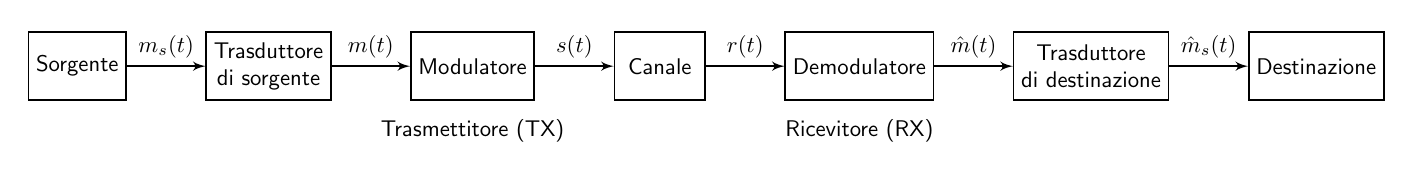
\begin{tikzpicture}[>=latex',font=\sffamily,semithick,scale=0.82, every node/.style={scale=0.82}]
            % Define the style for the blocks
            %\tikzstyle{block} = [draw, rectangle, minimum height=3em, minimum width=4em]
            \tikzstyle{block} = [rectangle, draw, minimum height=3em, minimum width=4em, text centered, align=center]

            % Nodes position
            \node [block] (source) {Sorgente};
            \node [block, right=1cm of source] (strasducer) {Trasduttore \\ di sorgente};
            \node [block, right=1cm of strasducer] (transmitter) {Modulatore};
            \node [block, right=1cm of transmitter] (channel) {Canale};
            \node [block, right=1cm of channel] (receiver) {Demodulatore};
            \node [block, right=1cm of receiver] (dtrasducer) {Trasduttore \\ di destinazione};
            \node [block, right=1cm of dtrasducer] (destination) {Destinazione};

            % Arrows
            \draw[->] (source) --   (strasducer) node[midway,above] {$m_s(t)$};
            \draw[->] (strasducer) --            (transmitter) node[midway,above] {$m(t)$};
            \draw[->] (transmitter) -- (channel) node[midway,above] {$s(t)$};
            \draw[->] (channel) -- (receiver) node[midway,above] {$r(t)$};
            \draw[->] (receiver) --  (dtrasducer) node[midway,above] {$\hat{m}(t)$};
            \draw[->] (dtrasducer) --               (destination) node[midway,above] {$\hat{m}_s(t)$};

            % Labels for modulation and demodulation
            \node[below of=transmitter, node distance=1cm] (modulation) {Trasmettitore (TX)};
            \node[below of=receiver, node distance=1cm] (demodulation) {Ricevitore (RX)};

            % Arrows for modulation and demodulation
            %$ \draw[->] (source) |- (modulation);
            %\draw[->] (modulation) -| (receiver);
            %\draw[->] (destination) |- (demodulation);
            %\draw[->] (demodulation) -| (transmitter);
        \end{tikzpicture}
    \end{adjustwidth*}
\end{figure}
% Now the explanation of the symbols in a table format
\begin{tabular}{ll}
    $m_s(t)$       & segnale fisico prodotto dalla sorgente (es. voce)                                      \\
    $m(t)$         & segnale elettrico ottenuto per trasduzione del segnale di sorgente (es. segnale audio) \\
    $s(t)$         & segnale modulato (trasmesso)                                                           \\
    $r(t)$         & segnale ricevuto                                                                       \\
    $\hat{m}(t)$   & segnale demodulato                                                                     \\
    $\hat{m}_s(t)$ & segnale trasdotto                                                                      \\
\end{tabular}
\\
\begin{enumerate}
    \item \textbf{Nodo di sorgente}: genera il messaggio (informazione) da comunicare.
    \item \textbf{Nodo di destinazione}: riceve il messaggio trasmesso.
    \item \textbf{Trasduttore di sorgente}: può convertire, ove necessario, il supporto fisico del segnale $m_s(t)$ così da generare un segnale elettrico opportuno per la trasmissione.



    \item \textbf{Trasmettitore}: converte il segnale elettrico \( m(t) \) in un nuovo segnale elettrico adatto per la trasmissione attraverso il canale di comunicazione a disposizione. Effettua sostanzialmente le seguenti operazioni:
          \begin{enumerate}
              \item Traslazione in frequenza (modulazione): fa sì che la occupazione di banda del segnale sia attorno a un opportuna frequenza centrale.
              \item Sagomatura: garantisce che la occupazione di banda sia quella ottimale e che non disturbi eventuali altre comunicazioni presenti nello stesso canale di comunicazione.
          \end{enumerate}

    \item \textbf{Canale di comunicazione}: permette il trasferimento del segnale \( s(t) \) dal nodo sorgente a quello di destinazione. Il canale di comunicazione prevede:
          \begin{enumerate}
              \item Un trasduttore di ingresso: converte il segnale elettrico \( s(t) \) in un segnale con supporto fisico compatibile con il mezzo trasmissivo (es. onda elettromagnetica per la trasmissione in aria libera per la trasmissione su fibra ottica, ecc.).
              \item Un mezzo trasmissivo: rappresenta il mezzo fisico su cui si propaga il segnale trasmesso (es. onda e vuoto per le onde elettromagnetiche o la fibra ottica per segnali luminosi).
              \item Un trasduttore di uscita: converte il segnale ricevuto tramite il mezzo trasmissivo in un segnale elettrico \( r(t) \).
          \end{enumerate}

    \item \textbf{Ricevitore}: trasforma il segnale \( r(t) \) in un segnale \( \hat{m}(t) \) traslando il segnale in frequenza (operazione di demodulazione) e operando un filtraggio. L'operazione di filtraggio si rende necessaria in quanto il segnale è generalmente una versione modificata del segnale \( s(t) \) per effetto della presenza di:
          \begin{itemize}
              \item rumore introdotto dal canale di comunicazione e dai dispositivi elettronici che compongono il ricevitore;
              \item distorsioni introdotte dal canale di comunicazione.
          \end{itemize}
          In ogni caso, il ricevitore deve effettuare una operazione di sagomatura inversa per ottenere il segnale \( \hat{m}(t) \) in modo che esso sia il più simile possibile al segnale \( m(t) \).

          Una condizione necessaria sul ricevitore è la seguente:
          \[
              \text{Se } r(t) = s(t) \text{ allora } \hat{m}(t) = m(t)
          \]

          Questa condizione deve essere interpretata nel seguente modo: se il segnale ricevuto è identico a quello trasmesso (assenza di disturbi introdotti dal canale di comunicazione) allora il segnale demodulato \( \hat{m}(t) \) deve essere identico a \( m(t) \).

          \subsection*{Banda Passante e Larghezza di Banda di un Canale di Comunicazione}
          Si può applicare il concetto di banda di un filtro.
          \pgfmathdeclarefunction{gauss}{2}{%
              \pgfmathparse{(1-exp(-((exp(-(abs((#1-x)/#2)*3-3)))^2)))}%
          }

          \begin{center}

              \begin{tikzpicture}
                  \begin{axis}[
                          title={Banda passante},
                          xlabel={Frequenza},
                          ylabel={Ampiezza},
                          xmin=0, xmax=30,
                          ymin=0, ymax=1,
                          xtick={10,15,20},
                          xticklabels={\( f_{\text{min}} \),\( f_0 \),\( f_{\text{max}} \)},
                          ytick={0.707,1},
                          yticklabels={-3dB,0dB},
                          legend pos=north east,
                          ymajorgrids=true,
                          grid style=dashed,
                      ]

                      \addplot[
                          color=red,
                          domain=0:30,
                          samples=100,
                          smooth,
                          thick,
                      ]
                      {gauss(15, 5)};

                      %\legend{Banda passante}

                  \end{axis}
              \end{tikzpicture}
          \end{center}

\end{enumerate}
\begin{itemize}
    \item $\text{Banda passante} \left\{ f \vert f_{\text{min}} \leq f \leq f_{\text{max}} \right\}$
    \item $\text{Larghezza di banda: } B = f_{\text{max}} - f_{\text{min}} $
    \item $\text{Frequenza centrale: } f_0 = \frac{f_{\text{max}} + f_{\text{min}}}{2}$
\end{itemize}



\subsection*{Canali a banda larga e a banda stretta}
Il concetto di banda larga o stretta è relativo alla frequenza centrale
\begin{itemize}
    \item \textbf{Banda larga}: $f_0 \leq 2B$
    \item \textbf{Banda stretta}: $f_0 > 2B$
\end{itemize}


Esempi:
\begin{enumerate}
    \item Doppino telefonico (banda larga):
          \begin{itemize}
              \item $f_0 = 2.45 KHz$
              \item $B = 3.7 KHz$
          \end{itemize}
    \item Canale radio (DVB-T, banda stretta)
          \begin{itemize}
              \item $f_0 = 400 MHz$
              \item $B = 8 MHz$
          \end{itemize}
\end{enumerate}

NB: Nonostante la larghezza di banda nel secondo caso sia maggiore che nel primo caso si ha che nel primo caso la banda è larga e nel secondo caso è stretta.

\subsection*{Il canale radio}
Il canale radio merita un po' di attenzione in quanto rappresenta il canale per le comunicazioni "wireless".



% Here we define the structure of the radio channel features
Le caratteristiche principali di un canale radio sono:
\begin{enumerate}
    \item È sempre un canale passa-banda.
    \item È tipicamente un canale a banda stretta.
    \item I trasduttori di canale sono delle \textbf{antenne} e queste devono avere delle dimensioni non inferiori a $\frac{\lambda}{10}$. Questo comporta dei limiti inferiori alle frequenze utilizzabili per la trasmissione radio.
\end{enumerate}

% The formula provided in the notes
\[
    \lambda = \frac{c}{f}
\]

% Radio channel frequency bands
\begin{tabular}{lll}
    LF (Low Frequency)     & 30 - 300 kHz   & Radiolocalizzazione marittima \\
                           & (1 - 10 km)    & e aeronautica                 \\
    MF (Medium Frequency)  & 300 - 3000 kHz & Radionavigazione e            \\
                           & (100 - 1000 m) & radiodiffusione               \\
    HF (High Frequency)    & 3 - 30 MHz     & Collegamenti a lunga distanza \\
                           & (10 - 100 m)   & (riflessione ionosferica)     \\
    VHF (Very High Freq.)  & 30 - 300 MHz   & Radiodiffusione               \\
                           & (1 - 10 m)     &                               \\
    UHF (Ultra High Freq.) & 300 - 3000 MHz & Servizi TV, telefonia mobile  \\
                           & (0.1 - 1 m)    &                               \\
    SHF (Super High Freq.) & 3 - 30 GHz     & TV satellitare, ponti radio   \\
                           & (1 - 10 cm)    &                               \\
\end{tabular}

% Notes on disturbances introduced in the communication channel

\subsection*{
    Disturbi introdotti dal canale di comunicazione
}
Il canale di comunicazione introduce distorsioni sul segnale trasmesso che possono essere descritte da trasformazioni deterministiche. In prima approssimazione tali distorsioni si possono assumere lineari e stazionarie.


Quindi, sotto questa ipotesi, il canale di comunicazione può essere visto come un filtro lineare e stazionario, che può introdurre quindi distorsioni lineari. La sua modellizzazione può essere a questo punto definita come segue:
\tikzset{
    block/.style = {draw, fill=white, rectangle,
            minimum height=3em, minimum width=3em},
    input/.style = {coordinate},
    output/.style = {coordinate},
    sum/.style = {draw, fill=white, circle, node distance=1cm}
}
% Block diagram for communication channel
\begin{center}
    \begin{tikzpicture}[auto, node distance=2cm,>=latex']
        \node [input, name=input] {};
        \node [block, right of=input] (channel) {c(t)};
        \node [output, right of=channel] (output) {};

        \draw [->] (input) -- node {s(t)} (channel);
        \draw [->] (channel) -- node {r(t)} (output);
        node [near end] {} (output);
    \end{tikzpicture}
\end{center}


dove \( c(t) \) è la risposta impulsiva del canale di comunicazione.

\bigskip
Il canale di comunicazione introduce inoltre un disturbo di tipo aleatorio noto come \textbf{rumore}. Tale rumore si può quindi modellare come un processo aleatorio di tipo additivo che quindi si somma alla componente utile del segnale ricevuto.
Quindi la modellizzazione completa di un canale di comunicazione può essere, in prima approssimazione, definita come segue:

% Complete block diagram with noise
\begin{center}
    \begin{tikzpicture}[auto, node distance=2cm,>=latex']
        \node [input, name=input] {};
        \node [block, right of=input] (channel) {c(t)};
        \node [draw, circle, right of=channel] (sum) {\(+\)};
        \node [output, right of=sum] (output) {};
        \node [block, below of=sum] (noise) {n(t)};

        \draw [->] (input) -- node {s(t)} (channel);
        \draw [->] (channel) -- node {} (sum);
        \draw [->] (noise) -- node {} (sum);
        \draw [->] (sum) -- node {r(t)} (output);
    \end{tikzpicture}
\end{center}

dove

\[
    r(t) = s(t) \ast c(t) + n(t)
\]

\textbf{Canale ideale}
\begin{align*}
                     & c(t) = \delta(t) \\
                     & n(t) = 0         \\
                    & r(t) = s(t)
\end{align*}


\subsection*{Sistemi di Comunicazione Analogici}
Un sistema di comunicazione si dice analogico quando sia \( m(t) \) che \( \hat{m}(t) \) sono segnali analogici.

Da notare che:
\begin{enumerate}
    \item Ovviamente anche \( m_s(t) \) e \( \hat{m}_s(t) \) sono segnali analogici in quanto differiscono rispettivamente da \( m(t) \) e \( \hat{m}(t) \) per un cambio del supporto fisico.
    \item \( s(t) \) e \( r(t) \) sono sempre segnali analogici in quanto il primo deve essere trasdotto in un segnale fisico e immesso nel mezzo trasmissivo ed il secondo si ottiene per trasduzione di un segnale fisico.
\end{enumerate}


\section*{Sistemi di Comunicazione Numerici}
Per definizione un sistema di comunicazione numerico è tale quando \( m_s(t) \) e \( \hat{m}_s(t)\) sono sequenze numeriche (\( m_s[n] \) e \( m_r[n] \)) e \( m(t) \) e \( \hat{m}(t) \) sono segnali numerici.

N.B. \( s(t) \) e \( r(t) \) continuano ad essere segnali analogici.

\begin{center}
    \begin{tikzpicture}[auto, node distance=2cm,>=latex']
        \node [input, name=input] {};
        \node [block, right of=input] (modulator) {\( p(t) \)};
        \node [output, right of=modulator] (output) {};

        \draw [->] (input) -- node {\( m_s[n] \)} (modulator);
        \draw [->] (modulator) -- node {\( m(t) \)} (output);
    \end{tikzpicture}
\end{center}
Dove
\( T_s \) è il periodo di segnalazione della sorgente e
\( m_s[n] \) è la sequenza generata dalla sorgente con periodo di sequenza \( T_s \),
Ogni simbolo di \( m_s[n] \) appartiene ad un alfabeto predefinito
\[ m_s[n] \in A_s ,  A_s = \alpha_1, \alpha_2, \ldots, \alpha_M\} ,  M \geq 2  \]La sequenza \( m_s[n] \) può essere vista come il risultato (realizzazione) del campionamento di un processo aleatorio.



\( M(t) \) è un processo aleatorio e \( M_s[n] \) è una V.A. estratta dal processo. \\
Si definisce la sequenza aleatoria di sorgente come
\[ \{ M_s[n] \in A_s, n = 0, \pm 1, \pm 2, \ldots \} \]
N.B. \( m_s[n] \) è una realizzazione di \( M[n] \).

Alla destinazione si definisce in maniera analoga la sequenza di destinazione
\[ \{ \hat{M}_s[n] \in A_s, n = 0, \pm 1, \pm 2, \ldots \} \]

Il segnale \( m(t) \) è ottenuto dalla sequenza aleatoria di sorgente tramite una operazione di modulazione che è del tutto equivalente alla operazione di interpolazione
\[ m(t) = \sum_{n=-\infty}^{+\infty} m_s[n]\cdot p(t - nT_s) \]
dove \( p(t) \) è l'impulso in trasmissione.

Ad esempio \( p(t) = \text{rect}\left(\frac{t}{T_s}\right) \).

Il tasso di erogazione della sorgente è definito come
\[ R_s \coloneqq \frac{1}{T_s} \]
che è il rate con cui escono i simboli apparentemente dall'alfabeto \( A_s \).

Se è presente una codifica binaria per rappresentare un simbolo dell'alfabeto \( A_s \) occorrono \( \log_2 M \) simboli binari,
per cui si definisce il tasso di errore binario come:
\[
    R_b \coloneqq \frac{\log_2 M}{T_s}
\]

\subsection*{Schema funzionale di un sistema di comunicazione numerico}
\begin{adjustwidth*}{-2.3cm}{-2cm}
    \begin{center}
        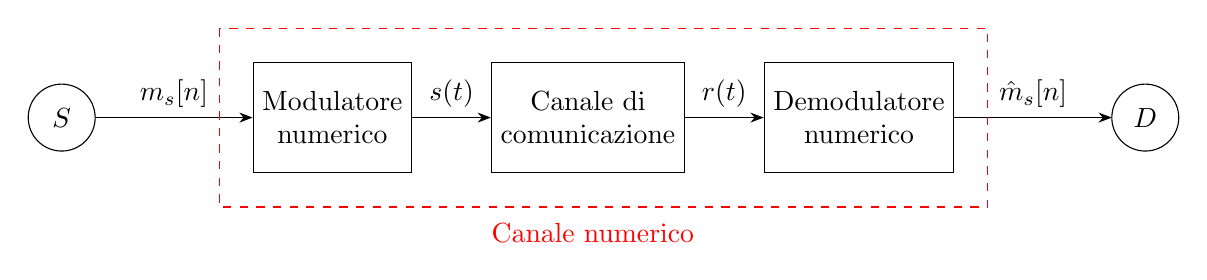
\begin{tikzpicture}[>=Stealth, block/.style={draw, rectangle}, scale=0.85]
            % Blocks
            \tikzstyle{block} = [rectangle, draw, text centered, minimum height=4em, align=center]

            \node[block] (mod) {Modulatore \\ numerico};
            \node[block, right=1cm of mod] (channel) {Canale di \\ comunicazione};
            \node[block, right=1cm of channel] (demod) {Demodulatore \\ numerico};

            % Nodes for connecting lines
            \coordinate[left=2cm of mod] (input);
            \coordinate[right=2cm of demod] (output);

            % Lines
            \draw[->] (input) -- node[above] {$m_s[n]$} (mod);
            \draw[->] (mod) -- node[above] {$s(t)$} (channel);
            \draw[->] (channel) -- node[above] {$r(t)$} (demod);
            \draw[->] (demod) -- node[above] {$\hat{m}_s[n]$} (output);

            % Dashed box
            \begin{scope}
                \draw[dashed, red] ($(mod.north west)+(-0.5,0.5)$) rectangle ($(demod.south east)+(0.5,-0.5)$);
            \end{scope}

            % Annotations
            \node[align=center, red, above right= -1cm and -6cm of demod.south east] (channel-label) {Canale numerico};

            % Circles
            \draw (input) ++(-0.5cm,0) circle (0.5cm) node {$S$};
            \draw (output) ++(0.5cm,0) circle (0.5cm) node {$D$};
        \end{tikzpicture}
    \end{center}
\end{adjustwidth*}
\begin{itemize}
    \item La coppia modulatore/demodulatore numerico può essere interpretata come un livello di trasduzione. Questo ci permette di vedere il sistema di comunicazione come un canale numerico tra \( S \) e \( D \).
    \item La sorgente genera una sequenza di simboli appartenenti all'alfabeto \( A_s \), che vogliamo trasferire al nodo di destinazione.
    \item Il modulatore numerico può essere visto come l'insieme del trasduttore di sorgente e del modulatore. Questo genera quindi il segnale \( s(t) \) analogico che può essere di tipo passa-basso (in banda base) o di tipo passa-banda (in banda passante).
    \item Il canale di comunicazione è sempre lo stesso (per segnali numerici e analogici).



    \item Il demodulatore numerico può essere visto come l'insieme del demodulatore e del trasformatore di destinazione. Esso produce la sequenza $\hat{m}_s[n]$ dal segnale $v(t)$.

\end{itemize}

Un canale numerico ideale produce:
\begin{equation}
    \hat{m}_s[n] = m_s[n] \quad \forall n
\end{equation}

In casi pratici un canale numerico non è mai ideale e per cui ha senso definire il suo comportamento e quindi le sue prestazioni.

\subsection*{Probabilità di transizione}
\begin{equation}
    P\{i|j\} \coloneqq P\{\hat{m}_s[n]=\alpha_i
    \ |\  m_s[n]=\alpha_j\}
\end{equation}

Un canale numerico è statisticamente caratterizzato quando sono note le $P\{i|j\}$ $\forall i,j$

Se le $P\{i|j\}$ non dipendono da $n$ allora il canale numerico si dice \textbf{stazionario}.

L'insieme delle $P\{i|j\}$ è parte di $M^2$ dove $M$ è la cardinalità dell'alfabeto $A_s$.

Per un canale ideale quindi:
\begin{align}
    P\{i|j\} & = 1 \quad \text{se } i=j      \\
    P\{i|j\} & = 0 \quad \text{se } i \neq j
\end{align}

N.B. Le $P\{i|j\}$ non dipendono solo dai disturbi introdotti dal canale di comunicazione, ma anche dalla modulazione impiegata, per cui esse legano contro delle prestazioni di tutto il sistema numerico.

% Qui potresti includere il disegno utilizzando l'ambiente tikzpicture se necessario
\subsection*{Misure delle prestazioni di un sistema di comunicazione numerico}

Le prestazioni di un sistema di comunicazione numerico sono associabili alla probabilità di errore di simbolo \(M\)-ario

\[
    P_E(M) \coloneqq P\{\hat{m}_s[n] \neq m_s[n]\}
\]

Se la \(P_E(M)\) non dipende da \(n\), allora il sistema di comunicazione è stazionario.

\subsection*{Quality of Service (QoS)}

La qualità del servizio per un sistema di comunicazione numerico è associabile alla probabilità di errore \(P_E(M)\). È ragionevole quindi pensare che si debba fissare una \(P_E(M)\) massima al di là della quale la QoS non è accettabile.

\[
    P_E(M) \leq P_{\text{max}}
\]

Esempio: per i servizi voce \(P_{\text{max}} = 10^{-3}\), mentre per i servizi dati \(P_{\text{max}} = 10^{-7}\).

\subsection*{Dualismo banda e potenza}

Aumentando la potenza del segnale in trasmissione si può fare in modo che la componente utile del segnale prevalga sulla componente di rumore. Questo intuitivamente tende a migliorare le prestazioni del sistema. La potenza però costa e comunque esistono dei limiti fisici o imposti che la limitano.

Lo stesso si può dire per la banda, si può dimostrare che all'aumentare della banda del segnale trasmesso si migliorano le prestazioni del sistema. Anche la banda però è una risorsa limitata.


\subsection*{Efficienza di potenza e efficienza spettrale}

Una modulazione si dice:
\begin{itemize}
    \item \textbf{efficiente in potenza}: quando la potenza trasmessa è bassa a fronte di un certo livello di prestazioni;
    \item \textbf{efficiente spettralmente}: quando la banda utilizzata è piccola a fronte di un certo livello di prestazioni.
\end{itemize}

Sfortunatamente i sistemi efficienti spettralmente non sono anche efficienti in potenza.

Vantaggi di un sistema di comunicazione rispetto ad un altro:
\begin{enumerate}
    \item Basso costo
    \item Sicurezza nella trasmissione di un messaggio
    \item Trasferimento aggregato di messaggi di natura diversa (multiplazione, audio, video, dati)
    \item Possibilità di utilizzare modulazioni e codifiche che rendono il sistema efficiente in potenza e/o spettralmente.
\end{enumerate}

Svantaggi:
\begin{enumerate}
    \item Generalmente la banda occupata da un segnale numerico è maggiore del corrispondente analogico
    \item Complessità, soprattutto per la sincronizzazione
\end{enumerate}


\section*{Modulazioni numeriche in banda base}

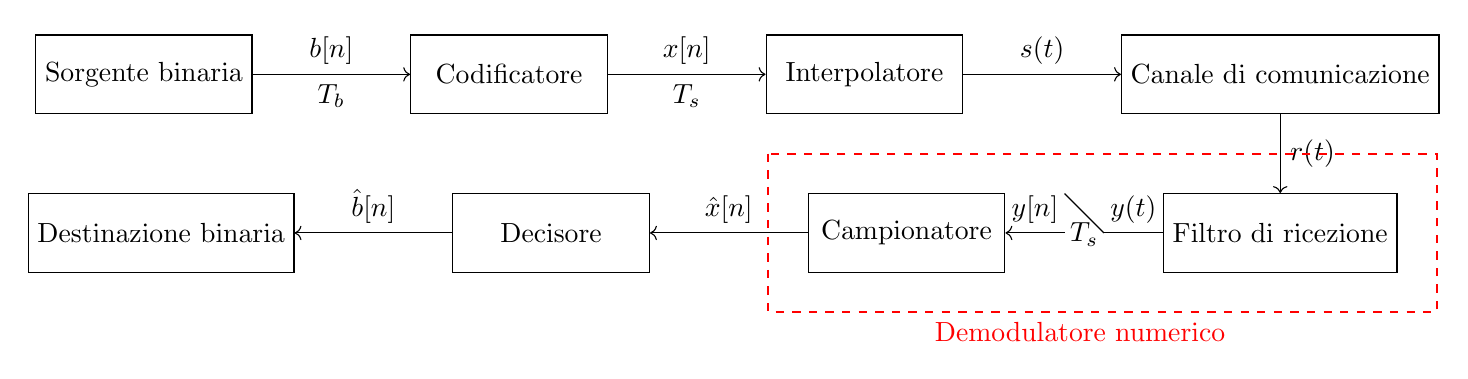
\begin{tikzpicture}[
    block/.style={rectangle, draw, minimum height=1cm, minimum width=2.5cm},
    node distance=1cm and 2cm,
    auto
]
    % Blocks
    \node[block] (source) {Sorgente binaria};
    \node[block, right=of source] (encoder) {Codificatore};
    \node[block, right=of encoder] (interp) {Interpolatore};
    \node[block, right=of interp] (channel) {Canale di comunicazione};
    \node[block, below=of channel] (filter) {Filtro di ricezione};
    \node[block, left=of filter] (sampler) {Campionatore};
    \node[block, left=of sampler] (decisor) {Decisore};
    \node[block, left=of decisor] (destination) {Destinazione binaria};

    % Arrows
    \draw[->] (source) -- (encoder) node[midway,above] {$b[n]$}  node[midway,below] {$T_b$};
    \draw[->] (encoder) -- (interp) node[midway,above] {$x[n]$}  node[midway,below] {$T_s$};
    \draw[->] (interp) -- (channel) node[midway,above] {$s(t)$};
    \draw[->] (channel) -- (filter) node[midway,right] {$r(t)$};
    %\draw[->] (filter) -- (sampler) node[midway,above] {$y(t)$};
    \draw[->] (sampler) -- (decisor) node[midway,above] {$\hat{x}[n]$};
    \draw[->] (decisor) -- (destination) node[midway,above] {$\hat{b}[n]$};
    
        % Draw the diagonal line
    % Dashed Boxes
    \draw ([xshift=0]filter.west) -- ([xshift=-0.75cm]filter.west) node[midway,above] {$y(t)$};
    \draw ([xshift=-0.75cm]filter.west) -- ([xshift=-1.25cm,yshift=0.5cm]filter.west) node[midway,below] {$T_s$};

    \draw[->] ([xshift=-1.25cm,yshift=0cm]filter.west) -- ++(sampler) node[midway,above] {$y[n]$};

    \draw[dashed, red, thick] ([xshift=-0.5cm,yshift=0.5cm]sampler.north west) rectangle ([xshift=0.5cm,yshift=-0.5cm]filter.south east);

     \node[align=center, red, above right= -1cm and -6cm of filter.south east] (channel-label) {Demodulatore numerico};

  
   

\end{tikzpicture}

La modulazione numerica è necessaria per poter trasmettere sequenze binarie attraverso un mezzo trasmissivo. In particolare, per adesso ci concentreremo su canali trasmissivi in banda base, come ad esempio il doppino telefonico o il cavo coassiale.

\begin{tikzpicture}
% Drawing the block diagram using TikZ package
% Note: You will need to adjust the positions of the blocks (nodes) and the arrows (paths) to match your notes.
\end{tikzpicture}

% Here you should draw the block diagram as per your notes using the TikZ package.
% Since the TikZ diagram could be quite complex, I will only outline the structure here.
\begin{enumerate}
    
\item \textbf{Codificatore}: trasforma sequenze di bit in simboli \( M \)-ari appartenenti a un alfabeto \( A_s \).

\item \textbf{Interpolatore}: modula impulsi tramite i simboli \( x[n] \) in ingresso per produrre una sequenza di impulsi \( s(t) \).
\[
s(t) = \sum_{k=-\infty}^{\infty} x[k] \cdot p(t - kT_s)
\]

\item \textbf{Canale di comunicazione}: sono assenti i trasduttori in quanto la propagazione nel mezzo trasmissivo è elettrica.

\item \textbf{Filtro di ricezione}: filtra componenti di rumore generate nel canale e compensa eventuali distorsioni.

\item \textbf{Campionatore}: preleva campioni dal segnale filtrato \( y(t) \).

\item \textbf{Decisore}: associa un simbolo dell'alfabeto \( A_s \) ad ogni campione.

\item \textbf{Decodificatore}: trasforma i simboli in sequenze binarie.
 
\end{enumerate}
\paragraph*{Codificatore}

\begin{itemize}
\item Deve essere sincrono con la sorgente
\[
T_s = T_b \log_2 M
\]
\[
R_s = \frac{1}{T_s} = \frac{1}{T_b \log_2 M}
\]


\item La sequenza di simboli generati dal codificatore viene considerata come un processo stazionario. Spesso i simboli trasmessi sono considerati equiprobabili:
\begin{equation*}
    P\{x[n]=\alpha_i\} = \frac{1}{M} \quad \forall i
\end{equation*}
\end{itemize}

\paragraph*{Interpolatore}

In un sistema di comunicazione numerico in banda base, l'interpolatore da solo svolge il compito di modulatore numerico, in quanto effettua la sagomatura, mentre non è prevista nessuna traslazione in frequenza. Il filtro sagomatore è realizzato tramite la generazione dell'impulso \( p(t) \). Infatti, si può pensare a \( P(f) \) come allo spettro del singolo impulso.
\begin{itemize}
    \item \(B_p\): banda dell'impulso \( p(t) \):
    \item \(E_p\): energia dell'impulso \( p(t) \):
\begin{equation*}
    E_p = \int_{-\infty}^{\infty} p(t)^2 \, dt = \int_{-\infty}^{\infty} |P(f)|^2 \, df
\end{equation*}
\end{itemize}





Data l'aleatorietà della sequenza di simboli \( x[k] \), \( s(t) \) deve essere interpretato come la realizzazione di un processo aleatorio \( S(t) \) stazionario.

Il processo \( S(t) \) ha una autocorrelazione \( R_s(\tau) \) ed una densità spettrale di potenza \( S_s(f) \).

Per cui è definita una potenza \( P_s \) ed una banda \( B_T \).


     L'energia media per bit può essere calcolata come:
 \begin{equation*}
    E_b = T_s P_b = \frac{E_s}{\log_2 M} = \frac{E_s}{B_t}
\end{equation*}
\begin{equation*}
    E_s \text{— energia media per simbolo}
\end{equation*}


\paragraph*{Demodulatore numerico}


Il demodulatore numerico produce una sequenza $\hat{x}[k]$ in modo tale da minimizzare la probabilità di errore. La probabilità di errore sul simbolo e sul bit sono:

\begin{align*}
    P_{E_s} &= P\{ \hat{x}[k] \neq x[k] \} \\
    P_{E_b} &= P\{ \hat{b}[n] \neq b[n] \} \quad \text{BEP (bit error probability)}
\end{align*}

\paragraph*{Canale numerico e prestazioni}
\begin{center}
\begin{tikzpicture}
\node (s) at (0,0) {\(x[k]\)};
\node[block] (encoder) at (3,0) {Canale numerico};
\node (r) at (6,0) {\(\hat{x}[k]\)};

\draw[->] (s) -- (encoder);
\draw[->] (encoder) -- (r);
\end{tikzpicture}
\end{center}




\begin{align*}
    x[k] &\in A_s & A_s &= \{\alpha_1, \alpha_2, \ldots, \alpha_M\}
\end{align*}

\begin{equation*}
    P_E(M) \coloneqq P\{\hat{x}[k] \neq x[k]\} = \sum_{i=1}^{M} \sum_{\substack{j=1 \\ j \neq i}}^{M} P\{\hat{x} = \alpha_i, x = \alpha_j\} = \sum_{i=1}^{M} \sum_{\substack{j=1 \\ j \neq i}}^{M} P\{\hat{x} = \alpha_i \ |\ x = \alpha_j\}\cdot P\{x=\alpha_j\}
\end{equation*}

Nel caso di simboli equiprobabili:

\begin{equation*}
    P_E(M) = \frac{1}{M} \sum_{i=1}^{M} \sum_{\substack{j=1 \\ j \neq i}}^{M} P\{\hat{x} = \alpha_i \ | \ x = \alpha_j\}
\end{equation*}

\paragraph*{Formato di modulazione equienergia}

\begin{equation*}
    E_s(i) = \int_{-\infty}^{\infty} s_i(t)^2 dt \quad s_i(t) \text{ è il segnale trasmesso in corrispondenza del simbolo } \alpha_i
\end{equation*}

Il formato di modulazione è equienergetico se
\begin{equation*}
    E_{s}(i) = E_{s} \quad \forall i
\end{equation*}

\paragraph*{Ortogonalità}

Il formato di modulazione è detto ortogonale se
\begin{equation*}
    \int_{-\infty}^{\infty} s_{i}(t) s_{j}(t) \, dt = 0 \quad \forall i \neq j
\end{equation*}

\paragraph*{Efficienza energetica}

Fissata una \( P_{E_{b}} \), l'efficienza energetica è definita come il valore
\begin{equation*}
    \eta_{P} \coloneqq \frac{1}{SNR} , \quad SNR \coloneqq \frac{P_{s}}{P_{n}}
\end{equation*}
che permette di ottenere tale \( BEP \).

Quando tanto maggiore è \( \eta_{P} \), tanto minore deve essere il \( SNR \) che garantisce una data \( BEP \).

\paragraph*{Efficienza spettrale}

L'efficienza spettrale è definita con il rapporto tra il tasso di erogazione binario e la banda di trasmissione
\begin{equation*}
    \eta_{b} \coloneqq \frac{R_{b}}{B_{T}} \quad \text{[bit/s/Hz]}
\end{equation*}

Quindi l'efficienza cresce quando a parità tasso di erogazione la banda utilizzata in trasmissione si riduce.

In termini di \( T_{s} \) e \( M \):
\begin{equation*}
    \eta_{b} = \frac{\log_2 M}{B_{T} T_{s}}
\end{equation*}


\section*{Pulse-amplitude modulation (PAM)}

La PAM nel caso generico è detta anche \( M \)-PAM o PAM \( M \)-aria dove con \( M \) si indica il numero di simboli presenti nell'alfabeto \( A_s \).

\begin{center}
    \begin{tikzpicture}
        \node (s) at (0,0) {\(x[k]\)};
        \node[block] (encoder) at (3,0) {\(p(t)\)};
        \node (r) at (6,0) {\(s(t)\)};

        \draw[->] (s) -- (encoder);
        \draw[->] (encoder) -- (r);
    \end{tikzpicture}
\end{center}

Proprietà che definiscono una \( M \)-PAM:

\begin{enumerate}
    \item \( s(t) \coloneqq \sum_{k=-\infty}^{+\infty} x[k]\cdot p(t - kT_s) \)
    \item Gli \( M \) valori \( (M \geq 2) \) che costituiscono l'alfabeto \( A_s = \{ \alpha_1, \alpha_2, \ldots, \alpha_M \} \) sono definiti come:
          \[ \alpha_i = 2i - 1 - M, \quad i = 1, 2, \ldots, M \]
\end{enumerate}

Esempio:

\( M=4 \) $\Rightarrow$ \( \alpha_1 = -3, \alpha_2 = -1, \alpha_3 = 1, \alpha_4 = 3 \)

\begin{center}
    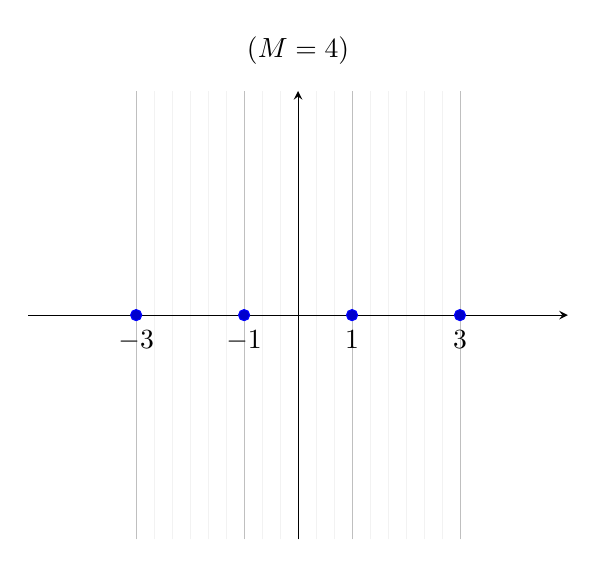
\begin{tikzpicture}
        \begin{axis}[
                title={\( (M=4) \)},
                xlabel={},
                ylabel={},
                xmin=-5, xmax=5,
                ymin=-4, ymax=4,
                grid=both,
                grid style={line width=.1pt, draw=gray!10},
                major grid style={line width=.2pt,draw=gray!50},
                minor tick num=5,
                axis lines=middle,
                minor tick style={draw=none},
                xtick={-3, -1, 1, 3},
                ytick=\empty,
            ]

            \addplot+[only marks] coordinates {
                    (-3, 0)
                    (-1, 0)
                    (1, 0)
                    (3, 0)
                };
        \end{axis}
    \end{tikzpicture}
\end{center}
\[
    E_s(i) = \int_{-\infty}^{+\infty} s_i^2(t) \, dt =  \int_{-\infty}^{+\infty} \alpha_i^2 \cdot p^2(t - kT_s) \, dt = \int_{-\infty}^{+\infty} (2i - 1 - M)^2 p^2(t) \, dt = (2i - 1 - M)^2 E_p
\]

Per \( M \) pari si ha \( A_s = \{ \pm 1, \pm 3, \ldots, \pm (M-1) \} \)

Per \( M \) dispari si ha \( A_s = \{ 0, \pm 2, \pm 4, \ldots, \pm (M-1) \} \)


I formati M-PAM di pi\`u largo impiego sono quelli dove $M$ è una potenza di 2.

Esempio:

$4$-PAM

sequenza = $\left\{ \begin{array}{l}
        x[-2] = -1, \\
        x[-1] = 1,  \\
        x[0] = -3,  \\
        x[1] = 1,   \\
        x[2] = 3    \\
    \end{array} \right.$

$p(t) = \text{rect}\left(\frac{t - T_s/2}{T_s}\right)$

\begin{center}
    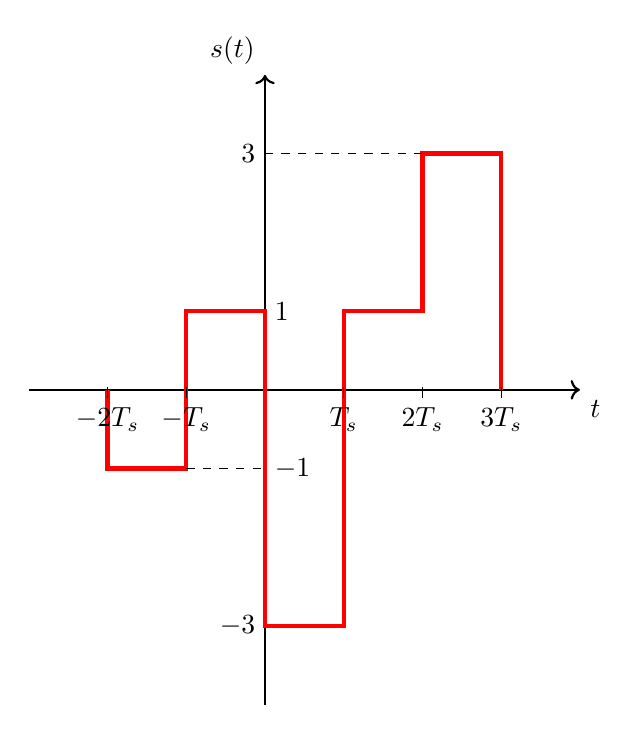
\begin{tikzpicture}
        % Assi
        \draw[thick,->] (-3,0) -- (4,0) node[anchor=north west] {$t$};
        \draw[thick,->] (0,-4) -- (0,4) node[anchor=south east] {$s(t)$};

        % Grafico a gradini
        \draw[ultra thick, red] (-2,0) -- (-2,-1) -- (-1,-1) -- (-1,1) -- (0,1) -- (0,-3) -- (1,-3) -- (1,1) -- (2,1) -- (2,3) -- (3,3) -- (3,0);

        % Tacche e etichette sull'asse delle x
        \foreach \x in {-2,2,3}
        \draw (\x cm,1pt) -- (\x cm,-3pt)
        node[anchor=north] {$\x T_s$};

        \draw (-1 cm,1pt) -- (-1 cm,-3pt)
        node[anchor=north] {$-T_s$};
        \draw (1 cm,1pt) -- (1 cm,-3pt)
        node[anchor=north] {$T_s$};

        % Linee tratteggiate
        \draw[dashed] (-1,-1) -- (0,-1);
        \draw[dashed] (2,3) -- (0,3);

        % Etichette
        \node at (0,1) [right] {$1$};
        \node at (0,-1) [right] {$-1$};
        \node at (0,3) [left] {$3$};
        \node at (0,-3) [left] {$-3$};
    \end{tikzpicture}
\end{center}

\subsection*{Proprietà derivate della M-PAM}
\begin{enumerate}
    \item Il valor medio di \( s(t) \) è zero per ogni \( t \):
          \begin{equation*}
              \mathbb{E}\left[ s(t) \right] = 0 \quad \forall t
          \end{equation*}
          \begin{equation*}
              \mathbb{E} \left[ \sum_{k=-\infty}^{+\infty} x[k] \ p(t-kT_s) \right] = \sum_{k=-\infty}^{+\infty} \mathbb{E}\left[x[k]\right]\ p(t-kT_s) = 0
          \end{equation*}
          \begin{equation*}
              \mathbb{E}\left[x[k]\right] = \frac{1}{M} \sum_{i=1}^{M} \alpha_i \mathbb{P}\{\alpha_i\} = \frac{1}{M} \sum_{i=1}^{M} (2i - 1 - M)
          \end{equation*}
          \begin{equation*}
              = \frac{2}{M} \sum_{i=1}^{M} i - 1 - M = \frac{2}{M} \frac{M(M+1)}{2} - (M+1) = 0
          \end{equation*}

    \item La densità spettrale di potenza invece è: \( S_s(f) \):
          \begin{equation*}
              S_s(f) = \frac{1}{T_s} S_x(f) \ |P(f)|^2
          \end{equation*}
          \begin{equation*}
              \text{dove } \sigma_x^2 = \mathbb{E}\left[ x\left[k\right]^2 \right] = \frac{(M-1)(M+1)}{3}
          \end{equation*}
\end{enumerate}

\[
    R_s(t,\tau) = \mathbb{E}\{s(t) \ s^*(t-\tau)\}
\]
\[
    = \mathbb{E} \left\{ \sum_{n=-\infty}^{+\infty} x\left[n\right] p(t - nT_s) \sum_{k=-\infty}^{+\infty} x^*\left[k\right] p^*(t - \tau - kT_s) \right\}
\]
\[
    = \sum_{n=-\infty}^{+\infty} \sum_{k=-\infty}^{+\infty} E\{x\left[n\right] x^*\left[k\right]\} \cdot p(t - nT_s) \cdot p^*(t - \tau - kT_s)
\]
\[
    = \sum_{n=-\infty}^{+\infty} \sum_{k=-\infty}^{+\infty} R_x\left[n-k\right] \cdot p(t - nT_s) \cdot p^*(t - \tau - kT_s)
\]

Imponendo \( n-k = m \) abbiamo che \( k = n-m \), quindi:

\[
    = \sum_{m=-\infty}^{+\infty} R_x[m] \sum_{n=-\infty}^{+\infty} p(t - nT_s) \cdot p^*(t - \tau - nT_s + mT_s)
\]

\paragraph*{Autocorrelazione media}

La funzione di autocorrelazione media \( \overline{R}_s(\tau) \) è:
\begin{align*}
    \overline{R}_s(\tau) & = \lim_{T\to\infty} \frac{1}{T} \int_{-\frac{T}{2}}^{\frac{T}{2}} R_s(t, \tau) dt                                                                   \\
    \overline{R}_s(\tau) & = \frac{1}{T_0} \int_{-\frac{T_0}{2}}^{\frac{T_0}{2}} R_s(t,\tau)dt \quad \text{se} \quad R_s(t,\tau) \quad \text{è periodico in} \quad t           \\
    \overline{R}_s(\tau) & = \sum_{m=-\infty}^{\infty} R_x[m] \frac{1}{T_s} \sum_{n=-\infty}^{\infty} \int_{-\frac{T_s}{2}}^{\frac{T_s}{2}} p(t-nT_s)p^*(t-\tau-nT_s+mT_s)dt   \\
                         & = \sum_{m=-\infty}^{\infty} R_x[m] \frac{1}{T_s} \sum_{n=-\infty}^{\infty}\int_{-\frac{T_s}{2}+nT_s}^{\frac{T_s}{2}+nT_s} p(t')p^*(t'-\tau+mT_s)dt' \\
                         & = \sum_{m=-\infty}^{\infty} R_x[m] \frac{1}{T_s} \int_{-\infty}^{\infty} p(t')p^*(t'-\tau+mT_s)dt'                                                  \\
                         & = \sum_{m=-\infty}^{\infty} R_x[m] \frac{1}{T_s} \int_{-\infty}^{\infty} P(f)[P(f)e^{-j2\pi f\tau}e^{j2\pi fmT_s}]^*df                              \\
                         & = \int_{-\infty}^{\infty} P(f)P^*(f)\frac{1}{T_s} \sum_{m=-\infty}^{\infty} R_x[m] e^{-j2\pi fmT_s}e^{j2\pi f\tau}df                                \\
                         & = \frac{1}{T_s} \int_{-\infty}^{\infty} |P(f)|^2 S_x(f)e^{j2\pi f\tau}df
\end{align*}


\[
    \overline{R}_s(\tau) = \frac{1}{T_s} TCF^{-1} \left[ |P(f)|^2 S_x(f) \right]
\]
\[
    \Rightarrow S_s(f) = \frac{1}{T_s} S_x(f) |P(f)|^2
\]

Nel caso in cui:
\begin{enumerate}
    \item $\mathbb{E} \{ x[n] \} = 0$
    \item $R_x[m] = \sigma_x^2 \delta[m]$
\end{enumerate}

Si ha che:
\[
    S_s(f) = \frac{\sigma_x^2}{T_s} |P(f)|^2
\]

In questo caso la $B_T$ coincide con quella del sagomatore $P(f)$.

Calcolo di $\sigma_x^2$:
\[
    \sigma_x^2 = \mathbb{E} \left[ (x - \mu_x)^2 \right] = \int_{-\infty}^{\infty} (x - \mu_x)^2 f_x(x) dx
\]
\[
    = \frac{1}{M} \sum_{i=1}^{M} (2i - 1 - M)^2
\]
\[
    = \frac{1}{M} \left[ 2 \sum_{i=1}^{M} i^2 + (1+M)^2 M - 4(1+M) \sum_{i=1}^{M} i \right]
\]

Sfruttando i seguenti risultati noti:
\[
    \sum_{i=1}^{n} i^2 = \frac{n(n+1)(2n+1)}{6}, \quad \sum_{i=1}^{n} i = \frac{n(n+1)}{2}
\]

Si ottiene:
\[
    \sigma_x^2 = \frac{M^2 - 1}{3}
\]

\[
    P_s = \frac{\sigma_x^2 E_p}{T_s} = \frac{M^2 - 1}{3} \frac{E_p}{T_s}
\]

\paragraph*{Efficienza Spettrale di una M-PAM}
\[
    \beta = \frac{R_b}{B_T} = \frac{\log_2 M}{T_s B_P}
\]
essendo \( B_T = B_P \),

L'efficienza spettrale aumenta con l'aumentare del numero di livelli. Sfortunatamente, come verrà dimostrato più avanti, l'efficienza in potenza diminuisce all'aumentare di \( M \).

\subsection*{PAM Binaria o BPSK (Binary Phase Shift Keying)}


\[
    s(t) = \sum_{k=-\infty}^{\infty} x[n] p(t - kT_s)
\]
con \( x[n] \in A_s = \{\pm 1\} \) (M = 2)

\[
    \Rightarrow T_B = T_s \quad (\log_2 2 = 1)
\]

Esempio con \( p(t) = \text{rect}\left(\frac{t-T_s/2}{T_s}\right) \)

% Drawing the binary PAM signal
\begin{center}

    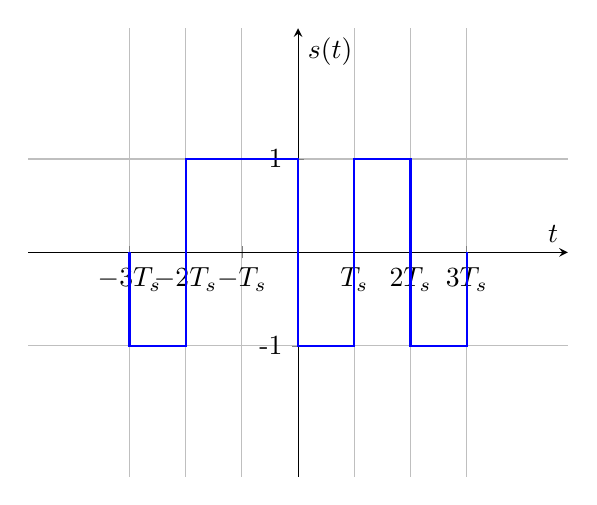
\begin{tikzpicture}
        \begin{axis}[
                xlabel = \( t \),
                ylabel = \( s(t) \),
                xtick={-3, -2, ..., 3},
                ytick={-1, 1},
                yticklabels={-1, 1},
                xticklabels={\(-3T_s\), \(-2T_s\), \(-T_s\), 0, \(T_s\), \(2T_s\), \(3T_s\)},
                ymin=-2, ymax=2,
                xmin=-4, xmax=4,
                axis lines=middle,
                enlargelimits=true,
                clip=false,
                grid=both
            ]
            \addplot+[const plot, no marks, thick] coordinates {(-3, 0) (-3,-1) (-2,-1) (-2,1) (0,-1) (1,1) (2,-1) (3,0)};
        \end{axis}
    \end{tikzpicture}
\end{center}
\[
    \text{Segnale PAM binario (o BPSK)}
\]

Il PAM Binario è un formato equiprobabile

% Energy calculation
\[
    E_{s_1} = \int_{-\infty}^{\infty} s_1^2(t) dt = \int_{-\infty}^{\infty} \left( +1 \right)^2 p^2(t) dt =  \int_{-\infty}^{\infty} \left( -1 \right)^2 p^2(t) dt = \int_{-\infty}^{\infty}  p^2(t) dt  = E_{s_2}
\]

\[
    E_{s_1} = E_{s_2} = \int_{-\infty}^{\infty} p^2(t) dt = E_p
\]

% Drawing the constellation diagram
\begin{center}

    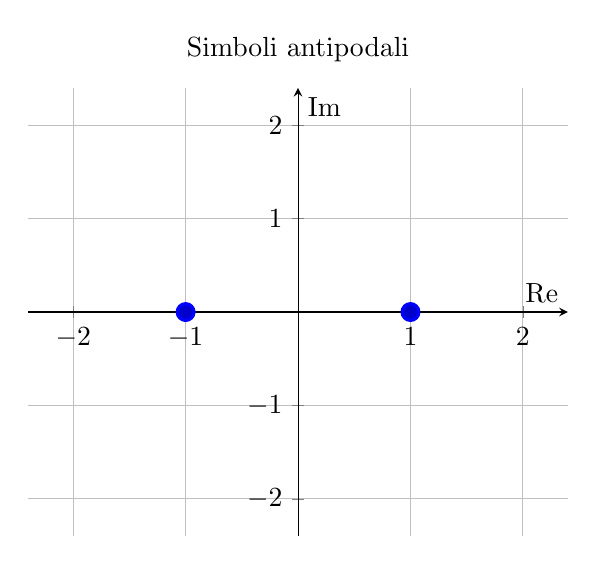
\begin{tikzpicture}
        \begin{axis}[
                title={Simboli antipodali},
                xlabel={Re},
                ylabel={Im},
                xmin=-2, xmax=2,
                ymin=-2, ymax=2,
                grid=both,
                axis lines=middle,
                enlargelimits=true
            ]
            \addplot+[only marks, mark size=3, very thick] coordinates {(1, 0) (-1, 0)};
            \node at (axis cs:1,0) [anchor=west] {};
            \node at (axis cs:-1,0) [anchor=east] {};
        \end{axis}
    \end{tikzpicture}
\end{center}



\begin{enumerate}
    \item $E\left[s(t)\right] = \dfrac{1}{2} \sum_{k=-\infty}^{+\infty} E[x_k] p(t-kT_s)
              = \sum_{k=-\infty}^{+\infty} \left(\dfrac{1}{2} (+1) + \dfrac{1}{2} (-1)\right) p(t-kT_s) = 0 \quad \text{se i simboli sono equiprobabili}$

    \item $S_s(t) = \dfrac{1}{T_b} |P(f)|^2 \quad \text{Densità spettrale di potenza}$

    \item $P_s = \dfrac{E_p}{T_b} \quad \text{Potenza media}$

    \item $B_T = B_P \quad \text{Banda}$

    \item $M_P = \dfrac{1}{T_bB_p}$
\end{enumerate}

\paragraph{Segnalazione ON-OFF}

È un tipo di PAM binaria con simboli appartenenti ad $A_s = \{0, 1\}$

e impulsi rettangolari  $p(t) = \text{rect}\left(\dfrac{t-T_b/2}{T_b}\right)$

\[
    s(t) = \sum_{k=-\infty}^{+\infty} x\left[k\right] \text{rect}\left(\dfrac{t-T_b/2-kT_b}{T_b}\right)
\]

\[
    \begin{cases}
        S_1(t) = 0                                            & \Rightarrow E_{S_1} = 0   \\
        S_2(t) = \text{rect}\left(\dfrac{t-T_b/2}{T_b}\right) & \Rightarrow E_{S_2} = T_b
    \end{cases}
\]


\begin{itemize}
    \item $
              E[S(t)] = \sum_{k=-\infty}^{+\infty} E[x[k]] p(t-kT_b) = \dfrac{1}{2}$
    \item $
              E_s = \dfrac{1}{2}E_{S_1} + \dfrac{1}{2}E_{S_2} = \dfrac{T_b}{2}
          $
    \item
          $
              P_s = \dfrac{E_s}{T_b} = \dfrac{1}{2}$
    \item $R_x[m] = C_x[m] + {\eta}_x^2 = \frac{1}{4} {\delta}[m] + \frac{1}{4}$

    \item $S_x(f) = TFS\left[ R_x[m] \right] = \frac{1}{4} + \frac{1}{4T_b} \sum_{m=-\infty}^{\infty} \delta\left(f - \frac{m}{T_b}\right)$
    \item $S_s(f) = \frac{1}{T_b} S_x(f)|P(f)|^2 = \frac{1}{T_b} \left( \frac{1}{4} + \frac{1}{4T_b} \delta(f) \right) T_b^2 \operatorname{sinc}^2(T_b f) = \frac{T_b}{4} \left( 1 + \frac{\delta(f)}{T_b} \right)\operatorname{sinc}^2(T_b f)$

    \item ${\eta}_b = \frac{\log_2{2}}{T_b B_p} = 2 \quad \text{e} \quad B_p = \frac{1}{2T_b} \text{ per la sinc}$
\end{itemize}



% Considerazioni
\subsection*{Considerazioni}
\begin{enumerate}
    \item L'efficienza spettrale della modulazione on-off è unitaria come nel caso della 2-PAM.
    \item Essendo la modulazione on-off di tipo unipolare (solo a valori positivi) questa può essere utilizzata su canali di comunicazione che, per loro natura, non possono sovrapporre segnali bipolari.
    \item La densità spettrale della on-off presenta un impulso di dirac nell'origine delle frequenze (alla continua) per cui il canale di trasmissione deve avere una risposta in frequenza che non sia nulla nell'origine.
\end{enumerate}

\section*{Prestazioni dei Sistemi di Comunicazione Numerici in Banda Base}
Nel valutare le prestazioni dei sistemi di comunicazioni numerici in banda base considereremo due fenomeni peggiorativi:
\begin{enumerate}
    \item Interferenza intersimbolo (ISI)
    \item Presenza di rumore
\end{enumerate}

Per il momento ignoriamo il rumore e ci concentriamo sul primo problema.

\subsection*{Interferenza intersimbolica (ISI)}
Il primo fenomeno è causato dalla non perfetta risposta in frequenza del canale di trasmissione e quindi dalle distorsioni lineari introdotte da questo.

\noindent
\begin{minipage}{.5\textwidth}
    \centering
    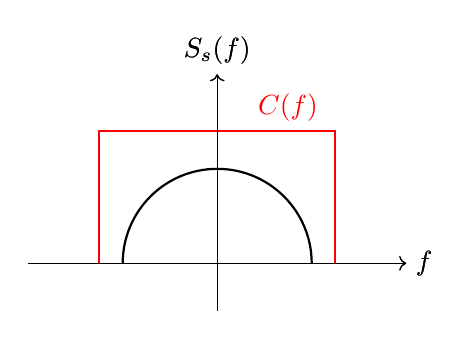
\begin{tikzpicture}[scale=0.6]
        % Canale ideale
        \draw[->] (-1,0) -- (4,0) node[right] {$f$}; % asse x
        \draw[->] (0,-1) -- (0,4) node[above] {$S_s(f)$}; % asse y
        \draw[thick, red] (-2.5,0) -- (-2.5,2.8) -- (2.5,2.8) -- (2.5,0); % rettangolo

        \draw[->] (-4,0) -- (4,0) node[right] {$f$}; % asse x
        \draw[->] (0,-1) -- (0,4) node[above] {$S_s(f)$}; % asse y
        \draw[thick, black] (-2,0) arc (180:0:2);

        \node[red, above] at (1.5,2.8) {$C(f)$};

        % Canale non ideale
        \begin{scope}[shift={(6,0)}] % sposta tutto a destra

        \end{scope}
    \end{tikzpicture}
    \\
    \textbf{Assenza di ISI:}
    \[
        y[k] = f(x[k])
    \]
    \\
\end{minipage}%
\begin{minipage}{.5\textwidth}
    \centering

    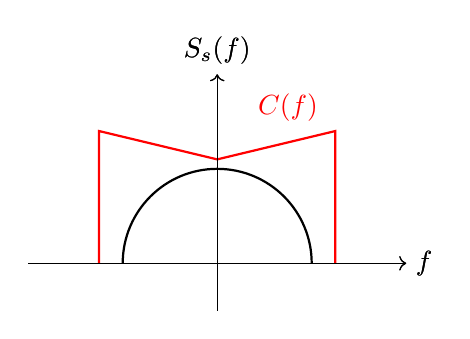
\begin{tikzpicture}[scale=0.6]
        % Canale ideale
        \draw[->] (-1,0) -- (4,0) node[right] {$f$}; % asse x
        \draw[->] (0,-1) -- (0,4) node[above] {$S_s(f)$}; % asse y
        \draw[thick, red] (-2.5,0) -- (-2.5,2.8) -- (0, 2.2) -- (2.5,2.8) -- (2.5,0); % rettangolo

        \draw[->] (-4,0) -- (4,0) node[right] {$f$}; % asse x
        \draw[->] (0,-1) -- (0,4) node[above] {$S_s(f)$}; % asse y
        \draw[thick, black] (-2,0) arc (180:0:2);

        \node[red, above] at (1.5,2.8) {$C(f)$};

        \begin{scope}[shift={(6,0)}] % sposta tutto a destra
        \end{scope}
    \end{tikzpicture}
    \\
    \textbf{Presenza di ISI:}
    \[
        y[k] = f(\dots, x[k-1], x[k], x[k+1], \dots)
    \]
    \\
\end{minipage}


Il risultato è che il campione estratto al ricevitore dal segnale ricevuto al k-esimo istante non dipende solo dal k-esimo simbolo.

\begin{center}
    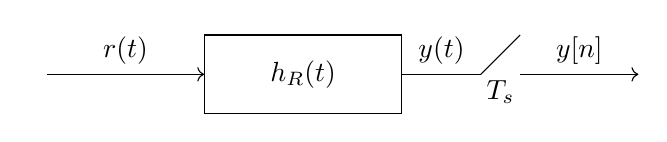
\begin{tikzpicture}[
            block/.style={rectangle, draw, minimum height=1cm, minimum width=2.5cm},
            node distance=1cm and 2cm,
            auto
        ]

        \node[block] (filter) {$h_R(t)$};
        \node[left=of filter] (channel) {};
        \node[right=of filter] (sampler) {};

        \draw[->] (channel) -- (filter) node[midway,above] {$r(t)$};

        \draw ([xshift=0]filter.east) -- ([xshift=1cm]filter.east) node[midway,above] {$y(t)$};
        \draw ([xshift=1cm]filter.east) -- ([xshift=1.5cm,yshift=0.5cm]filter.east) node[midway,below, yshift=-0.2cm] {$T_s$};

        \draw[->] ([xshift=1.5cm,yshift=0cm]filter.east) -- ++(1.5cm,0) node[midway,above] {$y[n]$};


    \end{tikzpicture}
\end{center}





Per ridurre gli effetti dell'ISI si devono considerare:
\begin{enumerate}
    \item il sagomatore in trasmissione \( p(t) \)
    \item la risposta impulsiva del canale \( c(t) \)
    \item il filtro in ricezione
\end{enumerate}

\begin{center}
    \begin{tikzpicture}[
            block/.style={rectangle, draw, minimum height=1cm, minimum width=2.5cm},
            node distance=1cm and 2cm,
            auto
        ]
        \node[block] (interpolatore) {$p(t)$};
        \node[left=of interpolatore] (tmp) {};
        \node[block, right= of interpolatore] (chan) {$c(t)$};
        \node[block, right= of chan] (filter) {$h_R(t)$};
        \node[right=of filter] (sampler) {};

        \draw[->] (channel) -- (interpolatore) node[midway,above] {$x[k]$};
        \draw[->] (interpolatore) -- (chan) node[midway,above] {$s(t)$};
        \draw[->] (chan) -- (filter) node[midway,above] {$r(t)$};

        \draw ([xshift=0]filter.east) -- ([xshift=1cm]filter.east) node[midway,above] {$y[k]$};
        \draw ([xshift=1cm]filter.east) -- ([xshift=1.5cm,yshift=0.5cm]filter.east) node[midway,below, yshift=-0.2cm] {$T_s$};

        \draw[->] ([xshift=1.5cm,yshift=0cm]filter.east) -- ++(1.5cm,0) node[midway,above] {$y[n]$};

        \draw[dashed, red, thick] ([xshift=-0.5cm,yshift=0.5cm]interpolatore.north west) rectangle ([xshift=0.5cm,yshift=-0.5cm]filter.south east);

        \node[align=center, red, above right= -1cm and -6cm of filter.south east] (channel-label) {$h(t)$};


    \end{tikzpicture}
\end{center}
\[
    h(t)=p(t) \ast c(t) \ast h_R(t)
\]

\paragraph*{Dimostrazione}
\[ Y(f) = R(f) \cdot H_R(f) = S(f) \cdot C(f) \cdot H_R(f) = \overline{X}(f) \cdot P(f) \cdot C(f) \cdot H_R(f) \]
\[ = \overline{X}(f) \cdot H(f) \quad  \text{dove} \quad H(f) = P(f) \cdot C(f) \cdot H_R(f) \]

\[ y(t) = \sum_{n=-\infty}^{+\infty} x[n] \cdot h(t - nT_s) \]

\[ y[k] = y(kT_s) = \sum_{n=-\infty}^{+\infty} x[n] \cdot h((k - n) \cdot T_s)  \]
\[ = x[k] \cdot h(0) + \sum_{\substack{n=-\infty \\ n \neq k}}^{+\infty} x[n]\cdot h((k - n) \cdot T_s) \]

Il secondo termine rappresenta la componente ISI.




\subsection*{Canale con ISI}

Un canale con banda \( B_c \) in generale introduce ISI. Ci sono due aspetti di cui ci occuperemo:

\begin{enumerate}
    \item Determinazione del \( T_s \) minimo che può essere adottato al fine di ottenere una sequenza campionata priva di ISI.
    \item Determinare le condizioni sotto le quali è possibile trasmettere un segnale M-PAM attraverso un canale non ideale in modo che non vi sia ISI nella sequenza campionata.
\end{enumerate}

Nel risolvere i due problemi riterremo \( c(t) \) fissata, e \( p(t) \) e \( h_R(t) \) variabili, in quanto determinabili dal progettista.

Un approccio non perseguibileconsiste nel trasmettere impulsi di durata finita e quindi con banda illimitata. Questo è in contrasto con la limitatezza messa a disposizione dal canale di trasmissione \( (B_c < \infty) \).

\(\Rightarrow\) Gli impulsi \( p(t) \) devono avere durata infinita.

\subsection*{Primo criterio di Nyquist per la trasmissione priva di ISI}

\[ h(kT_s) =
    \begin{cases}
        1, & \text{se } k=0      \\
        0, & \text{se } k \neq 0
    \end{cases}
    \quad \text{(Dominio del tempo)}
\]

\[ \sum_{k=-\infty}^{+\infty} H\left(f-\frac{k}{T_s}\right) = T_s \quad \forall f \quad \text{(Dominio della frequenza)} \]




\paragraph*{Dimostrazione}
Il primo criterio di Nyquist nel dominio del tempo garantisce l'assenza di ISI in quanto
\[ y[k] = x[k] \cdot h(0) + \sum_{\substack{n=-\infty \\ n \neq k}}^{+\infty} x[n] \cdot h((n-k)T_s) = x[k] \cdot h(0) \]
dove il secondo termine è nullo e non vi è ISI se \( h[n] = \delta[n] \).

La relazione in frequenza si ottiene come trasformazione
\[ h[k] = \delta[k] \quad \Longleftrightarrow \quad \overline{H}(f) = 1 \quad \forall f \]
\[ \overline{H}(f) = \frac{1}{T_s} \sum_{k=-\infty}^{+\infty} H\left(f - \frac{k}{T_s}\right) = 1 \quad \forall f \]
\[ \sum_{k=-\infty}^{+\infty} H\left(f - \frac{k}{T_s}\right) = T_s \quad \forall f \]

\subsection*{Trasmissione priva di ISI}
Supponiamo sia assegnato un canale a banda rigorosamente limitata con banda \( B_c \).
\[ C(f) = 0 \quad \text{per} \quad |f| > B_c \]
e supponiamo che \( B_T = B_c \), ovvero che il segnale trasmesso occupa tutta la banda messa a disposizione dal canale.
Allora si verificano le seguenti:
\begin{enumerate}
    \item Non è possibile in alcun modo eliminare l'ISI quando \( T_s < \frac{1}{2B_c} \).


          \paragraph*{Dimostrazione:}

          Quando \( T_s < \frac{1}{2B_c} \)

          \begin{tikzpicture}[scale=0.5]
              \draw[->] (-15,0) -- (15,0) node[right] {\( f \)};
              \draw[->] (0,-1) -- (0,7) node[above] {\( \overline{H}(f) \)};

              % Triangles
              \draw (-11,0) -- (-8,3) -- (-5,0);
              \draw[dashed, red] (-5,-1) -- (-5,4);
              \draw[dashed, red] (-3,-1) -- (-3,4);
              \draw (-3,0) -- (0,3) -- (3,0);
              \draw[dashed, red] (3,-1) -- (3,4);
              \draw[dashed, red] (5,-1) -- (5,4);
              \draw (5,0) -- (8,3) -- (11,0);

              \node at (-12,1.5) {\( \cdots \)};
              \node at (12,1.5) {\( \cdots \)};
          \end{tikzpicture}

          Esistono degli intervalli di frequenza dove \( \overline{H}(f) = 0 \) per cui non può mai accadere che \( \overline{H}(f) = 1 \) \( \forall f \)

          \bigskip

    \item Il più piccolo valore di \( T_s \) che permette di eliminare l'\( ISI \) è

          \( T_s^{(min)} = \frac{1}{2B_c} \)

          \bigskip

          \( f_s^{(max)}\) = \( \frac{1}{T_s^{(min)}} = 2B_c = f_N \) \quad (frequenza di Nyquist)

          \bigskip

          \begin{tikzpicture}[scale=0.5]
              \draw[->] (-15,0) -- (15,0) node[right] {\( f \)};
              \draw[->] (0,-1) -- (0,7) node[above] {\( \overline{H}(f) \)};

              % Triangles
              \draw (-9,0) -- (-6,3) -- (-3,0);
              \draw (-3,0) -- (0,3) -- (3,0);
              \draw (3,0) -- (6,3) -- (9,0);

              \node at (-10,1.5) {\( \cdots \)};
              \node at (10,1.5) {\( \cdots \)};
              \
          \end{tikzpicture}

          Non esistono intervalli di frequenza dove \( \overline{H}(f) = 0 \)

          \bigskip

    \item Nel caso valga la condizione \( T_s = \frac{1}{2B_c} \), allora l'unica funzione di trasferimento che permette di eliminare completamente l'\( ISI \) è

          \[ H(f) = \frac{1}{2B_c} \text{rect}\left(\frac{f}{2B_c}\right) \quad \Leftrightarrow \quad h(t) = \text{sinc}(2B_c t) \]





          \paragraph*{Dimostrazione:}

          \begin{center}

              \begin{tikzpicture}[scale=1]
                  \begin{axis}[
                          axis lines=middle,
                          xlabel={$f$},
                          ylabel={$H(f)$},
                          xtick={-4, -2, 2, 4},
                          xticklabels={$-2B_c$, $-B_c$, $B_c$, $2B_c$},
                          ytick={100},
                          yticklabels={},
                          ymin=-0.2, ymax=2,
                          xmin=-8, xmax=8,
                          %every axis x label/.style={at={(ticklabel* cs:1.05)}, anchor=west,},
                          %every axis y label/.style={at={(ticklabel* cs:1.05)}, anchor=south,},
                          xmajorgrids=false,
                          ymajorgrids=false,
                          clip=false
                      ]

                      % Draw the rectangle
                      \draw [thick] (axis cs:-2,0) rectangle (axis cs:2,0.4);

                      % Add the summation formula
                      \node [red]at (axis cs:7,0.6) {$\sum_{k=-\infty}^{\infty} H(f - \frac{k}{T_s})$};

                      % Draw the dashed lines
                      \draw [dashed, red] (axis cs:-6,0.4) -- (axis cs:-6,0);

                      \draw [dashed, red] (axis cs:-8,0.4) -- (axis cs:-2,0.4);
                      \draw [dashed, red] (axis cs:2,0.4) -- (axis cs:8,0.4);

                      \draw [dashed, red] (axis cs:6,0.4) -- (axis cs:6,0);

                  \end{axis}
                  \
              \end{tikzpicture}
          \end{center}

          Si nota anche che la funzione $\text{sinc}(2Bt)$ si annulla quando $t = \frac{k}{2B}$ con $k \neq 0$ per cui
          \[
              h[kT_s] = \text{sinc} \left(2B_c\cdot\frac{k}{2B_c}\right) = \text{sinc}(k) = \left\{
              \begin{array}{ll}
                  1 & \text{se } k=0    \\
                  0 & \text{se } k\neq0
              \end{array}
              \right.
          \]
\end{enumerate}


\textbf{Limiti di applicabilità della funzione di trasferimento rettangolare:}

\begin{enumerate}
    \item Realizzabilità di una funzione di trasferimento rettangolare: risposte in frequenza ideali come quella rettangolare non sono fisicamente realizzabili (Criterio di Paley-Wiener).
    \item Piccoli errori di campionamento provocano un ISI molto grande poiché la funzione $\text{sinc}(2B_ct)$ decresce molto lentamente.
\end{enumerate}

Un errore è nel campionatore induce un ISI grande in quanto si sommano molte contributi!




\begin{figure}[ht]
    \centering
    \begin{center}
        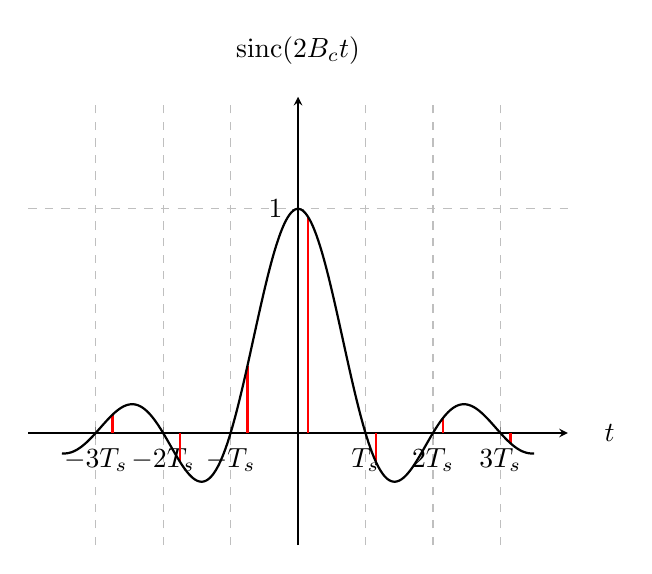
\begin{tikzpicture}
            \begin{axis}[
                    axis lines=middle,
                    xlabel={$t$},
                    ylabel={$\text{sinc}(2B_c t)$},
                    xtick={-3, -2, -1, 0, 1, 2, 3},
                    xticklabels={$-3T_s$, $-2T_s$, $-T_s$, $0$, $T_s$, $2T_s$, $3T_s$},
                    ytick={1},
                    ymin=-0.5, ymax=1.5,
                    xmin=-4, xmax=4,
                    every axis x label/.style={at={(ticklabel* cs:1.05)}, anchor=west,},
                    every axis y label/.style={at={(ticklabel* cs:1.05)}, anchor=south,},
                    xmajorgrids=true,
                    ymajorgrids=true,
                    grid style=dashed,
                    clip=false,
                    no markers,
                    samples=1000,
                    domain=-3.5:3.5
                ]


                \draw [thick, red] (axis cs:-2.75,0) -- (axis cs:-2.75,0.082);
                \draw [thick, red] (axis cs:-1.75,0) -- (axis cs:-1.75,-0.13);
                \draw [thick, red] (axis cs:-0.75,0) -- (axis cs:-0.75,0.30);

                \draw [thick, red] (axis cs:0.15,0) -- (axis cs:0.15,0.965);

                \draw [thick, red] (axis cs:1.15,0) -- (axis cs:1.15,-0.125);
                \draw [thick, red] (axis cs:2.15,0) -- (axis cs:2.15,0.07);
                \draw [thick, red] (axis cs:3.15,0) -- (axis cs:3.15,-0.045);


                % Define sinc function
                \addplot+[thick, black, smooth, unbounded coords=jump] {sin(deg(pi*x))/(pi*x)};
                \addplot+[thick, black, smooth] coordinates {(0, 1)};

                % Add the red vertical line at t=0

            \end{axis}
        \end{tikzpicture}
    \end{center}
    \caption*{Un errore $\epsilon$ nel campionatore induce un ISI grande in quanto si sommano molti contributi. In rosso l'errore $\epsilon$ del compionatore.}
    %\label{fig:my_label} % Optional, for referencing the figure
\end{figure}



Rilassando la condizione $T_s > \frac{1}{2B_c}$, ovvero ammettendo

\[ T_s > \frac{1}{2B_c} \]

si ottiene il seguente effetto:

\begin{center}

    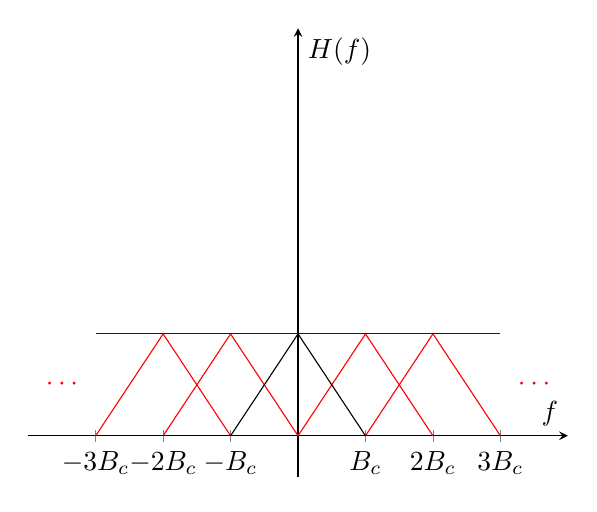
\begin{tikzpicture}[scale=1]
        \begin{axis}[
                axis lines=middle,
                xlabel={$f$},
                ylabel={$H(f)$},
                xtick={-6, -4, -2, 2, 4, 6},
                xticklabels={$-3B_c$, $-2B_c$, $-B_c$, $B_c$, $2B_c$, $3B_c$},
                ytick={100},
                yticklabels={},
                ymin=-0.2, ymax=2,
                xmin=-8, xmax=8,
                %every axis x label/.style={at={(ticklabel* cs:1.05)}, anchor=west,},
                %every axis y label/.style={at={(ticklabel* cs:1.05)}, anchor=south,},
                xmajorgrids=false,
                ymajorgrids=false,
                clip=false
            ]

            \node[red] at (-7,0.25) {\( \cdots \)};

            \draw[red] (-6,0) -- (-4,0.5) -- (-2,0);
            \draw[red] (-4,0) -- (-2,0.5) -- (0,0);

            \draw[red] (0,0) -- (2,0.5) -- (4,0);
            \draw[red] (2,0) -- (4,0.5) -- (6,0);

            \node[red] at (7,0.25) {\( \cdots \)};

            \draw[blue] (-6,0.5) -- (6,0.5);

            \draw (-2,0) -- (0,0.5) -- (2,0);


        \end{axis}
    \end{tikzpicture}
\end{center}

La sovrapposizione permette di definire una classe di infinite funzioni di trasferimento che soddisfano il primo criterio di Nyquist.

In questo caso però $B_c > \frac{1}{2T_s}$, per cui al punto di $T_s$ c'è bisogno di una banda disponibile nel canale che è maggiore di quella che occorre con la funzione di trasferimento rettangolare.

\subsection*{Filtro a coseno rialzato}

% Define the piecewise function
\[ H_{rc}(f) =
    \begin{cases}
        T_s                                                                                                          & \text{if } 0 \leq |f| \leq \frac{1-\alpha}{2T_s}                  \\
        \frac{T_s}{2} \left[ 1 - \sin\left(\frac{\pi T_s}{\alpha} \left( |f| - \frac{1}{2T_s} \right)\right) \right] & \text{if } \frac{1-\alpha}{2T_s} < |f| \leq \frac{1+\alpha}{2T_s} \\
        0                                                                                                            & \text{if } |f| > \frac{1+\alpha}{2T_s}
    \end{cases}
\]

con $0 < \alpha < 1$.

\begin{center}

    \definecolor{myblue}{RGB}{30,144,255}
    \definecolor{myred}{RGB}{178,34,34}
    \begin{tikzpicture}
        \begin{axis}[
                axis lines=middle,
                xlabel={$f$},
                ylabel={$H_{RC}(f)$},
                xtick={-0.5, 0.5},
                xticklabels={$\frac{-1}{2T_s}$, $\frac{1}{2T_s}$},
                ytick={0.5},
                yticklabels={$T_s/2$},
                ymin=0, ymax=1.5,
                xmin=-1, xmax=1,
                every axis x label/.style={at={(ticklabel* cs:1.05)}, anchor=west,},
                every axis y label/.style={at={(ticklabel* cs:1.05)}, anchor=south,},
                xmajorgrids=false,
                ymajorgrids=false,
                clip=false,
                no markers,
            ]

            % Draw the ideal filter response (black box)
            \draw [thick] (axis cs:-0.5,0) -- (axis cs:-0.5,1) -- (axis cs:0.5,1) -- (axis cs:0.5,0);

            % Draw the realistic filter response for alpha = 0.5 (blue line)
            % \addplot [myblue, thick, smooth, domain=-1:1] {0.5+0.5*cos(deg(pi*x))};
            \addplot [myblue, thick, smooth, domain=-0.75:0.-0.25] {0.5 * (1 + cos(deg(pi*(abs(x)-0.25)/0.5)))};
            \addplot [myblue, thick, smooth, domain=0.25:0.75] {0.5 * (1 + cos(deg(pi*(abs(x)-0.25)/0.5)))};


            % Draw the realistic filter response for alpha = 1 (red dashed line)
            \addplot [myred, thick, dashed, smooth, domain=-1:1] {0.5-0.5*sin(deg(pi*(abs(x)-0.5))};

            % Add annotations for alpha values
            \node[myblue] at (axis cs:0.75,0.8) {$\alpha=0.5$};
            \node at (axis cs:-0.75,0.8) {$\alpha=0$};
            \node[myred] at (axis cs:0.9,0.2) {$\alpha=1$};

            % Add black dot at intersection
            \node[circle,fill,inner sep=1.5pt] at (axis cs:0,0.5) {};

        \end{axis}
    \end{tikzpicture}
\end{center}
\subsection*{Propriet\`a}
\begin{enumerate}
    \item Quando \( \alpha = 0 \) il coseno rialzato coincide con la funzione di trasferimento rettangolare
    \item La banda \( B_H \) \`e direttamente ottenibile da \( B_H = \frac{1+\alpha}{2T_S} \)
\end{enumerate}

La \( h_{RC}(t) \) \`e calcolabile in forma chiusa:

\[ h_{RC}(t) = \sin\left(\frac{t}{T_S}\right) \frac{\cos\left(\frac{\alpha \pi t}{T_S}\right)}{\left(1- \frac{2\alpha t}{T_S}\right)^2}  \]

\[ h_{RC}(kT_S) = \delta[k] \]

\begin{itemize}
    \item Soddisfa il criterio di Nyquist nel tempo, per cui garantisce l'assenza di ISI
    \item Decresce per \( t \rightarrow \infty \) come \( \frac{1}{|t|^3} \) per \( \alpha > 0 \) quindi molto pi\`u velocemente del caso \( \alpha = 0 \) (rettangolare)
\end{itemize}




\subsection*{Eccesso di banda e efficienza spettrale dei sistemi \( M-PAM \) con coseno rialzato}

Dato:
\[ p(t) \otimes c(t) \otimes h_R(t) = h_{RC}(t) \]
dove \( \otimes \) indica la convoluzione, $p(t)$ il sagomatore in trasmissione, $c(t)$ la risposta impulsiva del canale , $h_R(t)$ il filtro in ricezione e \( h_{RC}(t) \) la risposta impulsiva del filtro a coseno rialzato, l'efficienza spettrale del canale di comunicazione numerico è:
\[ \eta_{B} = \frac{\log_2M}{B_T T_s} = \frac{\log_2M}{B_H T_s} = \frac{\log_2M}{ T_s} \frac{2T_s}{1+\alpha} = \frac{2\log_2M}{1+\alpha}\]

Considerazioni:
\begin{itemize}
    \item L'efficienza spettrale, a parità di \( M \), decresce al crescere del coefficiente di roll-off (\( \alpha \)).
    \item La robustezza del sistema di comunicazione numerico all'ISI aumenta al crescere di \( \alpha \).
\end{itemize}

C'è quindi un trade-off tra robustezza all'ISI e efficenza spettrale, e i valori ottimali si trovano in corrispondenza di \( \alpha \simeq 0.4 \) .

\[ \text{Eccesso di banda richiesto dall'adozione del coseno rialzato:} \]
\[ \Delta B_{H} = B_{H} - \frac{1}{2T_s} = \frac{\alpha}{2T_s} \]



\subsection*{Prestazioni di un sistema di comunicazione numerico in banda base in presenza di rumore}

\paragraph*{Capacità di canale}

La capacità \( C \) di un canale di comunicazione è definita come il massimo valore che può assumere il tasso binario di segnalazione \( R_b = \frac{1}{T_b} \) al variare di tutte le possibili coppie modulatore/demodulatore, sotto il vincolo che la probabilità di errore sia esattamente nulla.


\[
    \begin{cases}
        C \coloneqq \max_{\{R_b\}} \\
        P_E(b) = P\{\hat{b}[n] \neq b[n]\} = 0
    \end{cases}
\]

La capacità di canale \( C \) si misura in bit/s ed è un numero non-negativo. Ovviamente, più è grande la capacità del canale e migliori sono le sue prestazioni.

\paragraph*{Capacità di canale con rumore gaussiano bianco additivo (AWGN)}

\begin{center}
    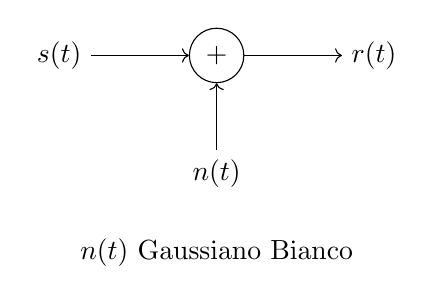
\begin{tikzpicture}
        \node (s) at (0,0) {\(s(t)\)};
        \node[draw, circle] (plus) at (2,0) {\(+\)};
        \node (n) at (2,-1.5) {\(n(t)\)};
        \node (r) at (4,0) {\(r(t)\)};

        \draw[->] (s) -- (plus);
        \draw[->] (n) -- (plus);
        \draw[->] (plus) -- (r);
        \node[below of=n, node distance=1cm] {\(n(t)\) Gaussiano Bianco};
    \end{tikzpicture}
\end{center}

In questo caso la capacità di canale può essere espressa in forma chiusa ed è in dipendenza dei parametri caratteristici del segnale trasmesso e del rumore.

\[
    C = B_T \log_2 \left( 1 + \frac{P_s}{N_0 B_T} \right) \quad \text{(Shannon)}
\]

Dove:
\begin{itemize}
    \item \( B_T \) = banda del segnale \( s(t) \)
    \item \( P_s \) = potenza media di \( s(t) \)
    \item \( \frac{N_0}{2} \) = DSP del rumore \( n(t) \) (costante essendo bianco)
\end{itemize}

Considerazioni:

\begin{enumerate}
    \item Fissato \( B_T \)
          \begin{align*}
              \lim_{\frac{P_s}{N_0} \to \infty} C & = 0       \\
              \lim_{\frac{P_s}{N_0} \to \infty} C & = +\infty
          \end{align*}

    \item Fissato \( \frac{P_s}{N_0} \)
          \begin{align*}
              \lim_{B_T \to \infty} C & = 0                              \\
              \lim_{B_T \to \infty} C & = \log_2 e \cdot \frac{P_s}{N_0}
          \end{align*}

    \item Riscrivendo la formula di Shannon utilizzando \( P_s = E_b R_b \)
          \[
              \frac{C}{B_T} = \log_2 \left( 1 + \frac{E_b}{N_0} \cdot \frac{R_b}{B_T} \right)
          \]
          Dove:
          \begin{itemize}
              \item \( E_b \) = energia per bit
              \item \( R_b \leq C \) (data la definizione di \( C \) come valore massimo di \( R_b \))
          \end{itemize}
\end{enumerate}

\paragraph*{Sistema di comunicazione numerico ideale}
Un sistema di comunicazione numerico è detto ideale se soddisfa le seguenti condizioni:
\begin{enumerate}
    \item \( R_b = C \)
    \item \( P_E(b) = 0 \)
\end{enumerate}

In queste condizioni è possibile mettere in relazione l'efficienza spettrale con il rapporto \( \frac{E_b}{N_0} \) (legato all
efficienza in potenza)

\[
    \eta_B = \log_2 \left( 1 + \frac{E_b}{N_0} \eta_B  \right) \quad \text{soggetto a} \quad  \eta_B = \frac{R_b}{B_T} = \frac{C}{B_T}
\]

\[
    \Rightarrow \frac{E_b}{N_0} = \frac{2^{\eta_B} - 1}{\eta_B} \quad \text{con} \quad \eta_B \geq 0
\]


\paragraph*{Considerazioni}

\begin{enumerate}
    \item
          $\lim_{\eta_B \to +\infty} \frac{2^{\eta_B } - 1}{\eta_B } = +\infty$


    \item $\lim_{\eta_B \to +\infty} \frac{2^{\eta_B } - 1}{\eta_B } = \ln{2} \quad (-1.6 \, \text{dB})$

\end{enumerate}


\subsection*{Ricezione ottima in presenza di rumore bianco}

Per il momento consideriamo solo gli effetti relativi al rumore.

\begin{center}
    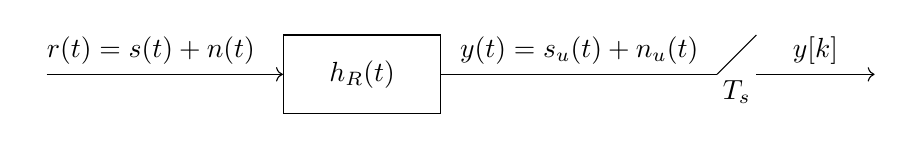
\begin{tikzpicture}[
            block/.style={rectangle, draw, minimum height=1cm, minimum width=2cm},
            node distance=3cm and 3cm,
            auto
        ]

        \node[block] (filter) {$h_R(t)$};
        \node[left=of filter] (channel) {};
        \node[right=of filter] (sampler) {};
        \draw[->] ([xshift=-3cm]filter.west) -- (filter.west) node[midway,above] {$r(t)=s(t)+n(t) \quad$};


        \draw ([xshift=0]filter.east) -- ([xshift=3.5cm]filter.east) node[midway,above] {$y(t)=s_u(t)+n_u(t)$};
        \draw ([xshift=3.5cm]filter.east) -- ([xshift=4cm,yshift=0.5cm]filter.east) node[midway,below, yshift=-0.2cm] {$T_s$};

        \draw[->] ([xshift=4cm,yshift=0cm]filter.east) -- ++(1.5cm,0) node[midway,above] {$y[k]$};
    \end{tikzpicture}
\end{center}
Dove \( s(t) \) è un segnale di forma nota e \( n(t) \) è un rumore additivo bianco

\[
    s_u(t) = s(t) \ast h_R(t), \quad n_u(t) = n(t) \ast h_R(t)
\]

\[
    y(T_s) = s_u(T_s) + n_u(T_s)
\]

Si definisce il rapporto segnale-rumore in uscita al filtro \( h_R(t) \) all'istante \( t = T_s \) come

\[
    SNR \coloneqq \frac{s_u^2(T_s)}{E[n_u^2(T_s)]}
\]

Si definisce ricevitore ottimo il filtro \( h_R(t) \) che massimizza l'SNR in uscita al filtro.

Nel caso di rumore bianco in ingresso il filtro ottimo prende il nome di \textbf{filtro adattato}

Problema:
\begin{enumerate}
    \item Derivare il filtro \( h_R(t) \) che massimizza l'SNR all'uscita.
    \item Determinare il valore massimo dell'SNR all'uscita.
\end{enumerate}


\paragraph*{Derivazione del filtro adattato}

L'SNR viene espressa come:
\[
    \text{SNR} = \frac{s_u^2(T_s)}{E[n_u^2(T_s)]}
\]

Calcoliamo i termini al numeratore e al denominatore della SNR.
\[
    s_u^2(T_s) = \left( \int_{-\infty}^{+\infty} s(\tau) h_R(T_s - \tau) d\tau \right)^2 = \left( \int_{-\infty}^{+\infty} S(f) H_R(f) e^{j2\pi fT_s} df \right)^2
\]

E l'energia del rumore all'uscita del filtro ricevitore sarà:
\[
    E[n_u^2(T_s)] = R_{n_u}(0)
\]

Dove:
\[
    R_{n_u}(\tau) = R_n(\tau) \ast h_R(\tau) \ast h_R(-\tau)
\]

E quindi per la potenza del rumore:
\[
    S_{n_u}(f) = S_n(f) \left| H_r(f) \right|^2 = \frac{N_0}{2} \left| H_R(f) \right|^2
\]

\[
    R_{n_u}(0) = \int_{-\infty}^{+\infty} S_{n_u}(f) df
\]

Sostituendo otteniamo l'SNR in funzione della risposta in frequenza del filtro ricevitore \( h_R(f) \):
\[
    \text{SNR} = \frac{\left( \int_{-\infty}^{+\infty} S(f) H_R(f) e^{j2\pi fT_s} df \right)^2}{\frac{N_0}{2} \int_{-\infty}^{+\infty} \left| H_R(f) \right|^2 df} = \frac{2}{N_0 E_{h_R}} \left( \int_{-\infty}^{+\infty} S(f) H_R(f) e^{j2\pi fT_s} df \right)^2
\]

Utilizzando la disuguaglianza di Schwarz si può dimostrare che $\int_{-\infty}^{+\infty} S(f) H_R(f) e^{j2\pi fT_s} df$ raggiunge il massimo valore quando:
\[
    H_R(f) e^{j2\pi fT_s} = S^*(f)
\]

Quindi:
\[
    H_R(f) = S^*(f) e^{-j2\pi fT_s}
\]

\[
    \boxed{h_R(t) = s(T_s - t)}
\]

Dalla espressione della risposta impulsiva \( h_R(t) \) si deduce il nome di \textbf{filtro adattato}, in quanto la sua risposta impulsiva è adattata al segnale in ingresso al filtro stesso.



Studiando il modulo della risposta in frequenza \( H_R(f) \) si deduce che il filtro tende ad amplificare le componenti frequenziali dove è presente il segnale e ad attenuare (o eliminare) le componenti frequenziali dove il contributo di segnale è scarso (o addirittura assente).

\[
    \left| H_R(f) \right| = \left| S(f) \right|
\]

La simbologia per indicare un filtro adattato è \( h_{FA}(t) \) o \( H_{FA}(f) \).

Esempio:

% Drawing the example signals using TikZ
\begin{tikzpicture}
    \draw[->] (-1,0) -- (5,0) node[right] {\(t\)};
    \draw[->] (0,-1) -- (0,2) node[above] {\(s(t)\)};
    \draw[dashed] (0,1) -- (1,1);
    \node at (0,1) [left] {\(1\)};
    \draw (0,0) -- (1,1) -- (1,0);
    \node at (1,0) [below] {\(T_s\)};
    \draw[->] (6,0) -- (12,0) node[right] {\(t\)};
    \draw[->] (7,-1) -- (7,2) node[above] {\(h_{FA}(t)\)};
    \draw (7,1) -- (8,0);
    \node at (8,0) [below] {\(T_s\)};
\end{tikzpicture}

Calcolo del \( SNR_{max} \)

Il valore del \( SNR_{max} \) si ottiene per definizione quando si utilizza il \( FA \).

\[
    SNR = \frac{2}{N_0 E_s} \cdot E_s^2 = \frac{2E_s}{N_0}
\]

Da notare che:

\begin{itemize}
    \item Il \( SNR \) non dipende dalla forma del segnale, ma solo dalla sua energia. Questo da spazio alla progettazione della forma del segnale indipendentemente dai risultati in termini di \( SNR \).
    \item Il massimo del \( SNR \) si ottiene per qualunque \( h_{FA}(t) = k \cdot s(T_s-t) \) con \( k \in \mathbb{R} \), infatti basta calcolare il $SNR$:
          \[ SNR = \frac{2}{N_0K^2 E_s} \cdot K^2 E_s^2 = \frac{2 E_s}{N_0} \]
\end{itemize}

Quindi, fattori di amplificazione e/o attenuazione non cambiano il risultato. Questo è abbastanza intuitivo in quanto un fattore costante di amplificazione opera allo stesso modo sul segnale utile e sul rumore per cui nel rapporto i contributi si elidono.

\paragraph*{Schema del ricevitore con filtro adattato}

Consideriamo la trasmissione di un simbolo:

\begin{center}
    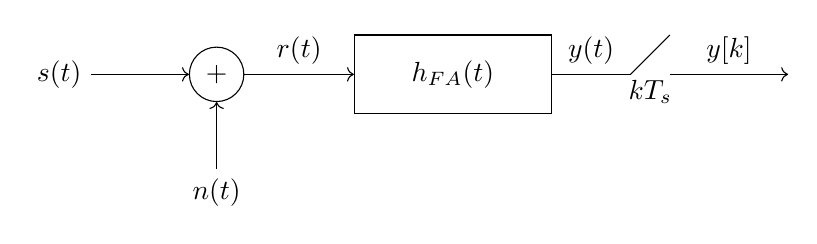
\begin{tikzpicture}[
            block/.style={rectangle, draw, minimum height=1cm, minimum width=2.5cm},
            node distance=1cm and 2cm,
            auto
        ]




        \node[block] (filter) {$h_{FA}(t)$};
        %\node[left=of filter] (channel) {};
        \node[right=of filter] (sampler) {};




        \node (s) at (-5,0) {\(s(t)\)};
        \node[draw, circle] (plus) at (-3,0) {\(+\)};
        \node (n) at (-3,-1.5) {\(n(t)\)};

        \draw[->] (s) -- (plus);
        \draw[->] (n) -- (plus);
        %\draw[->] (plus) -- (channel);

        \draw[->] (plus) -- (filter) node[midway,above] {$r(t)$};

        \draw ([xshift=0]filter.east) -- ([xshift=1cm]filter.east) node[midway,above] {$y(t)$};
        \draw ([xshift=1cm]filter.east) -- ([xshift=1.5cm,yshift=0.5cm]filter.east) node[midway,below, yshift=-0.2cm] {$kT_s$};

        \draw[->] ([xshift=1.5cm,yshift=0cm]filter.east) -- ++(1.5cm,0) node[midway,above] {$y[k]$};


    \end{tikzpicture}
\end{center}

\[ s(t) = \alpha \cdot p(t-nTs) \]
\[ h_{FA}(t) = k \cdot p(T_s - t) \]
\[ y(t) = s_u(t) + n_u(t) \]

Caratteristiche di \( s_u(t) \) e \( n_u(t) \):

\[ s_u(t) = s_u(t) \ast h_{FA}(t) = k \cdot \alpha \cdot p(t) \ast p(T_s - t) \]
\[ = k \cdot \alpha \int_{-\infty}^{\infty} p(\tau) p(\tau - (t - T_s)) d\tau = k \cdot \alpha \cdot C_p (t - T_s) \]
\[ C_p(t) = \int_{-\infty}^{\infty} P(\tau) P(\tau - t) d\tau \quad \text{(Autocorrelazione dell'impulso sagomatore)}
\]

\textbf{Esempio:}\\
La funzione rettangolare:
\[ s(t) = \text{rect}\left(\frac{t - \frac{T_s}{2}}{T_s}\right) \]

La risposta unitaria:
\[ s_u(t) = C_s(t - T_s) = T_s\cdot \left( 1 - \frac{\left| t - T_s \right|}{T_s} \right) \text{rect}\left(\frac{t - T_s}{2T_s}\right) \]
\noindent
\begin{minipage}{.5\textwidth}
    \centering

    % Diagrammi usando TikZ
    \begin{tikzpicture}
        \begin{axis}[
                axis lines = middle,
                xlabel = \( t \),
                ylabel = \( s(t) \),
                xtick = {1},
                xticklabels={$T_s$},
                ytick = {1},
                ymin = 0, ymax = 3.5,
                xmin = 0, xmax = 2.5,
                every axis x label/.style={at={(current axis.right of origin)},anchor=west},
                every axis y label/.style={at={(current axis.above origin)},anchor=south}
            ]
            \addplot+[const plot, no marks, thick] coordinates {(0,1) (1,1) (1,0)};
        \end{axis}
    \end{tikzpicture}
\end{minipage}%
\begin{minipage}{.5\textwidth}
    \centering
    \begin{tikzpicture}
        \begin{axis}[
                axis lines = middle,
                xlabel = \( t \),
                ylabel = \( s_u(t) \),
                xtick = {1, 2},
                xticklabels={$T_s$, $2T_s$},
                ytick = {1},
                yticklabels={$T_s$},
                ymin = 0, ymax = 2.5,
                xmin = 0, xmax = 2.5,
                every axis x label/.style={at={(current axis.right of origin)},anchor=west},
                every axis y label/.style={at={(current axis.above origin)},anchor=south}
            ]
            \draw[dashed] (0, 1) -- (1, 1) -- (1,0);
            \addplot+[sharp plot, no marks, thick] coordinates {(0,0) (1,1) (2,0)};
        \end{axis}
    \end{tikzpicture}
    \\
\end{minipage}


\[ n_u(t) = n(t) \ast h_{FA}(t) \]
\[ n(t) = \text{rumore bianco Gaussiano additivo (AWGN)} \]
\[ E[n(t)] = 0 \]
\[ R_n(\tau) = \sigma_n^2 \delta(\tau) = \frac{N_0}{2} \delta(\tau) \]
\[ n(\overline{t}) = \text{variabile aleatoria con densità di probabilità } f_N(n) = \frac{1}{\sqrt{2\pi\sigma_n^2}} e^{-\frac{n^2}{2\sigma_n^2}} = \frac{1}{\sqrt{N_0}} e^{-\frac{n^2}{N_0}} \]
Essendo il filtro in ricezione un filtro lineare e stazionario, \( n_u(t) \) è un rumore Gaussiano, additivo e stazionario.
\[ E[n_u(t)] = 0 \]
\[ R_{n_u}(\tau) = R_n(\tau) \ast h_{FA}(\tau) \ast h_{FA}(-\tau) = \frac{N_0}{2} C_{h_{FA}}(\tau)  \]
\[
    C_{h_{FA}}(\tau) = \text{autocorrelazione di } h_{FA}(t)
\]
\[ S_{n_u}(f) = \frac{N_0}{2} |H_{FA}(f)|^2 \]
\[ P_{n_u} = \frac{N_0}{2} E_{H_{FA}} = \frac{N_0}{2} E_p k^2 \]

È importante capire se i campioni di rumore sono tutti loro correlati o meno.
\[
    E[n_u[k]n_u[n]] = 0 \quad \forall k \neq n \quad \text{(incorrelazione)}
\]
N.B. la si può scrivere così poiché
\(E[n_u[k]] = 0\)

Questo vuol dire che
\[
    R_{n_u}[kT_s] = 0 \quad \forall k \neq 0
\]

\[
    R_{n_u}[nT_s] = \frac{N_0}{2} C_p[kT_s] = 0 \Rightarrow C_p[kT_s] = 0
\]


Dobbiamo ricordare che il segnale utile in ingresso al filtro adattato è ottenuto tramite il modulatore in trasmissione per cui è la funzione \( p(t) \) che determina la sagoma (forma) del segnale \( s(t) \).

\begin{enumerate}
    \item Impulso rettangolare
          \[
              p(t) = \text{rect}\left(\frac{t-T_s/2}{T_s}\right)
          \]

          \[
              C_p(\tau) = T_s \left(1 - \frac{|\tau|}{T_s}\right) \text{rect}\left(\frac{\tau}{2T_s}\right)
          \]

          \[
              R_{n_u}(\tau) = k \frac{N_0}{2} C_p(\tau)
          \]

          \[
              R_{n_u}(nT_s) =
              \begin{cases}
                  \frac{k^2 N_0 T_s}{2} & \text{se } k = 0    \\
                  0                     & \text{se } k \neq 0
              \end{cases}
              \Rightarrow
              \text{campioni di rumore incorrelati} \Rightarrow \text{indipendenti (Gaussiani)}
          \]
          \begin{center}
              \begin{tikzpicture}
                  \draw[->] (-3.5,0) -- (3.5,0) node[right] {$\tau$};
                  \draw[->] (0,-0.5) -- (0,2) node[above] {$C_p(\tau)$};
                  \draw[scale=1,domain=-1.5:1.5,smooth,variable=\x] plot ({\x},{1.5-abs(\x)});
                  \draw (1.5,0.1) -- (1.5,-0.1) node[below] {$T_s$};
                  \draw (-1.5,0.1) -- (-1.5,-0.1) node[below] {$-T_s$};
                  \draw (0.1,1.5) -- (-0.1,1.5) node[left] {$T_s$};
              \end{tikzpicture}

          \end{center}
    \item Impulso a radice di coseno rialzato
          \[
              P(f) = \sqrt{H_{RC}(f)}
          \]

          \begin{align*}
              S_{n_u}(f)    & = k^2 \frac{N_0}{2} |P(f)|^2 = k^2 \frac{N_0}{2} H_{RC}(f) \\
              R_{n_u}(\tau) & = k^2 \frac{N_0}{2} h_{RC}(\tau)                           \\
              R_{n_u}(nT_s) & = \begin{cases}
                                    \frac{k}{2} N_0, & k = 0    \\
                                    0,               & k \neq 0
                                \end{cases} \quad
              \text{N.B. la $h_{RC}(\tau)$ ha la sinc che si annulla in multipli di $T_s$.}
          \end{align*}

\end{enumerate}


\paragraph{SNR per bit all'ingresso del ricevitore}

Il SNR per bit è un parametro utile per determinare le prestazioni di una ricevitore in quanto tiene in considerazione quantità energetiche sia del segnale utile che del rumore
\[
    SNR_b = \frac{E_b}{N_0}
\]
\[
    E_b \coloneqq P_s T_b = E\left[x^2[k]\right]T_b \quad \text{Energia per bit} \]
\[
    \frac{N_0}{2} = S_n(f)
    \Rightarrow SNR_b = \frac{E\left[ x[k]\right]}{N_0 R_b}, \quad R_b = \frac{1}{T_b}
\]

\paragraph{Decisore ottimo e criterio della massimo verosimiglianza}

Il decisore deve mappare i campioni $y[k]$ in simboli dell'alfabeto. I campioni $y[k]$ sono statisticamente indipendenti l'uno dall'altro. Questo è dimostrato dal fatto che:

\[
    y[k] = s_u[k] + n_u[k]
    \quad
    \text{dove } s_u(k) \text{ e } n_u(k) \text{ sono indipendenti}
\]


%\draw[->] (source) -- (encoder) node[midway,above] {$b[n]$}  node[midway,below] {$T_b$};
\begin{center}
    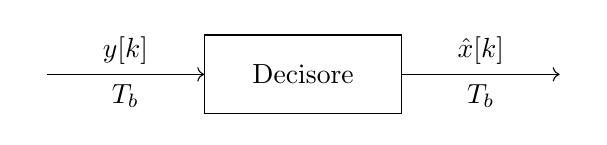
\begin{tikzpicture}[
            block/.style={rectangle, draw, minimum height=1cm, minimum width=2.5cm},
            node distance=1cm and 2cm,
            auto
        ]
        \node[block] (filter) {Decisore};
        \node[left=of filter] (channel) {};
        \node[right=of filter] (sampler) {};

        \draw[->] (channel) -- (filter) node[midway,above] {$y[k]$}  node[midway,below] {$T_b$};
        \draw[->] (filter) -- (sampler) node[midway,above] {$\hat{x}[k]$}  node[midway,below] {$T_b$};
    \end{tikzpicture}
\end{center}

Quindi si può concludere che $\hat{x}[k] \in A_s $ può essere deciso in base alla sola conoscenza di $y[k]$. Questa decisione si dice di tipo "ad un sol colpo" (one-shot detector).

\paragraph{Decisione a minima probabilità di errore}

\begin{itemize}
    \item Probabilità di errore sul simbolo
          \(
          P_E(M) \coloneqq P\{\hat{x}[k] \neq x[k]\}
          \)
    \item
          Criterio di ottimalità: minimizzazione della $P_E(M)$

\end{itemize}

Derivazione del decisore ottimo:
\[
    x \coloneqq \hat{x}[k], \quad y \coloneqq y[k], \quad n_u \coloneqq n_u[k], \quad \hat{x} = \hat{x}[k]
\]

\paragraph{Criterio a massima probabilità a posteriori e minima probabilità di errore}
Con
MAP si intende l'acronmo di Maximum A-posteriori Probability
\[
    \hat{x} = \arg\max_{i=1,\ldots,M} P(x=\alpha_i|y)
\]

Viene associato ad un osservato $y$ il simbolo dell'alfabeto $\hat{x}$ tale che sia massima la probabilità a posteriori (condizionata) che quel simbolo sia stato trasmesso.

Se il decisore adotta il criterio MAP allora la probabilità di errore sul simbolo è minima.


\paragraph{Dimostrazione}

Definiamo
\(
R(i) \coloneqq \left\{ y \in \mathbb{R} : \hat{x} = \alpha_i \right\}, \quad i = 1,\ldots,M
\)
come la "zona di decisione" del simbolo $\alpha_i$, ovvero l'insieme dei valori di $y$ per cui si decide per il simbolo $\alpha_i$.

\[
    P\{x = \alpha_i | y\} = \frac{f_Y(y | \hat{x} = \alpha_i) P\{x = \alpha_i\}}{f_Y(y)} \quad (\text{Bayes})
\]

\[
    P_E(M) = P\{\hat{x} \neq x\} = 1 - P\{\hat{x} = x\} = 1 - \sum_{i=1}^M P\{\hat{x} = \alpha_i, x = \alpha_i\}
\]

\[
    = 1 - \sum_{i=1}^M P\{\hat{x} = \alpha_i | x = \alpha_i\} P\{x = \alpha_i\} =
\]

\[
    = 1 - \sum_{i=1}^M P\{x = \alpha_i\} P\{y \in R(i) | x = \alpha_i\}
\]

\[
    = 1 - \sum_{i=1}^M P\{x = \alpha_i\} \int_{y \in R(i)} f_Y(y | x = \alpha_i) dy
\]

\[
    = 1 - \sum_{i=1}^M \int_{y \in R(i)} P\{x = \alpha_i\} f_Y(y | x = \alpha_i) dy
\]

\[
    = 1 - \sum_{i=1}^M \int_{y \in R(i)} f_Y(y) P\{x = \alpha_i | y\} dy
\]

Per minimizzare la $P_E(M)$ devo scegliere le $R(i)$ in modo tale che osservato $y$ sia massima la probabilità a posteriori relativa al simbolo $i$-esimo.

Si osserva che se le probabilità a priori sono identiche
\[
    P\{x = a_i\} = \frac{1}{M}, \quad i=1,\ldots,M
\]
allora, dato che $f_Y(y)$ non dipende da $i$:
\[
    \hat{x} = \arg \max_{i=1,\ldots,M} \left\{ \frac{1}{M} \frac{f_Y(y | x = \alpha_i)}{f_Y(y)} \right\} = \arg \max_{i=1,\ldots,M} f_Y(y | x = \alpha_i)
\]


La funzione $f_Y(y|x=\alpha_i)$ viene detta anche \textbf{funzione di verosimiglianza}

In pratica il criterio di minima probabilità di errore (o massima probabilità a posteriori) coincide con il criterio di massima verosimiglianza quando le probabilità a priori $P\{x=\alpha_i\}$ sono identiche.
Nel caso di AGWN
\[
    y = s_u + n_u = \alpha_i + n_u, \quad n_u \in \mathcal{N}(0,\sigma_{n_u}^2)
\]
\[
    f_Y(y|x = \alpha_i) = f_{n_u}(y - \alpha_i)
\]
\[
    = \frac{1}{\sqrt{2\pi\sigma_{n_u}^2}} e^{-\frac{(y-\alpha_i)^2}{2\sigma_{n_u}^2}}
\]

\[
    \hat{x} = \underset{i=1,\ldots,M}{\mathrm{argmax}} \frac{1}{\sqrt{2\pi\sigma_{n_u}^2}} e^{-\frac{(y-\alpha_i)^2}{2\sigma_{n_u}^2}} = \underset{i=1,\ldots,M}{\mathrm{argmin}}  (y - \alpha_i)^2
\]

\[
    \boxed{
        \hat{x} = \underset{i=1,\ldots,M}{\mathrm{argmin}} \{ |y-\alpha_i| \}
    } \quad \text{(minimo della distanza euclidea)}
\]


Il decisore ottimo coincide con la scelta del simbolo a distanza euclidea minima dall'osservato.

Le zone di decisione sono quindi stabilite dalla regola di quantizzazione uniforme.

Questo significa che il decisore può essere realizzato con un quantizzatore uniforme.


\paragraph{Ricevitore ottimo per un sistema di comunicazione PAM}

Per un sistema di comunicazione PAM con simboli equiprobabili, il ricevitore ottimo secondo il criterio a minima probabilità di errore è il seguente:

\begin{center}
    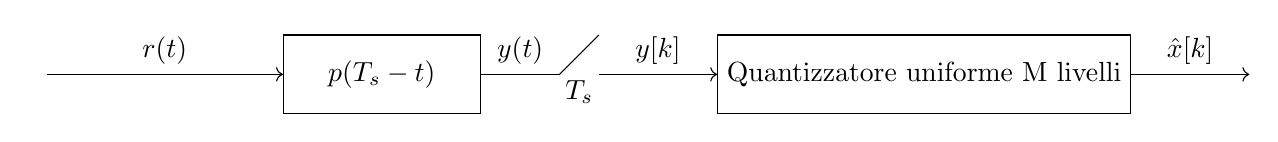
\begin{tikzpicture}[
            block/.style={rectangle, draw, minimum height=1cm, minimum width=2.5cm},
            node distance=3cm and 3cm,
            auto
        ]

        \node[block] (filter) {$p(T_s - t)$};
        \node[left=of filter] (channel) {};
        \node[right=of filter] (sampler) {};
        \node[block, right=of filter](quantizzatore) {Quantizzatore uniforme M livelli};

        \draw[->] (channel) -- (filter) node[midway,above] {$r(t)$};

        \draw ([xshift=0]filter.east) -- ([xshift=1cm]filter.east) node[midway,above] {$y(t)$};
        \draw ([xshift=1cm]filter.east) -- ([xshift=1.5cm,yshift=0.5cm]filter.east) node[midway,below, yshift=-0.2cm] {$T_s$};

        \draw[->] ([xshift=1.5cm,yshift=0cm]filter.east) -- ++(quantizzatore) node[midway,above] {$y[k]$};

        \draw[->] (quantizzatore.east) -- ++(1.5cm,0) node[midway,above] {$\hat{x}[k]$};

    \end{tikzpicture}
\end{center}

\begin{figure}
    \centering
    \begin{center}
        \begin{tikzpicture}[scale=0.75]
            % Assi
            \draw[thick,->] (-6,0) -- (6,0) node[anchor=north west] {};
            \draw[thick,->] (0,-5) -- (0,5) node[anchor=south east] {};

            % Grafico a gradini
            \draw[ultra thick, red] (-4,-3) -- (-2,-3) -- (-2,-1) -- (0,-1) -- (0,1) -- (2,1) -- (2,3) -- (4,3);

            % Tacche e etichette sull'asse delle x
            \foreach \x in {-4,-2,2,4}
            \draw (\x cm,1pt) -- (\x cm,-3pt)
            node[anchor=north] {$\x$};


            % Linee tratteggiate
            \draw[dashed, red] (-4,0) -- (-4,-3);
            \draw[dashed, red] (-2,-1) -- (-2,0);

            \draw[dashed, red] (4,0) -- (4,3);
            \draw[dashed, red] (2,1) -- (2,0);
            \draw[dashed, red] (2,3) -- (0,3);
            \draw[dashed, red] (-2,-3) -- (0,-3);

            % Etichette
            \node at (0,1) [left] {$1$};
            \node at (0,-1) [right] {$-1$};
            \node at (0,3) [left] {$3$};
            \node at (0,-3) [right] {$-3$};
        \end{tikzpicture}
    \end{center}
    \caption*{Esempio di una 4-Pam, con quantizzatore uniforme a 4 livelli}
\end{figure}

\paragraph{Probabilità di errore di bit e di simbolo}

\[
    P_E(b) = P\{\hat{b}[k] \neq b[k]\} \quad \text{bit}
\]

\[
    P_E(M) = P\{\hat{x}[k] \neq x[k]\} \quad \text{simbolo}
\]

\[
    P_E(M) = P_E(b) \quad \text{solo quando l'alfabeto } A_s \text{ è composto da soli due simboli}
\]
Vale però sempre che:
\[
    \frac{P_E(M)}{\log_2 M} \leq P_E(b) \leq \frac{M/2}{M-1} P_E(M)
\]

\paragraph{Codifica di Gray}

Sia \( A_s = \{\alpha_1, \ldots, \alpha_M\} \) dove
\[
    \alpha_i = 2i - M - 1 \quad i = 1, \ldots, M
\]

La codifica di Gray associa stringhe di bit ai simboli dell'alfabeto in modo che le stringhe di bit relative a due simboli consecutivi differiscano al più per un bit.

Nel caso di SNR sufficientemente elevato \( (> 10 dB) \), l'evento errore consiste generalmente nel decidere per uno dei simboli dell'alfabeto adiacenti a quello trasmesso.

Utilizzando quindi la codifica di Gray e in condizioni di SNR elevato, un errore su un simbolo \( M-ario \) ogni \( N \) simboli  \( M-ari \) si traduce in un errore su una sola cifra binaria ogni \( N \) simboli \( M-ari \), cioè ogni \( N \log_2 M \) cifre binarie, quindi:

\[
    P_E(b) \approx \frac{P_E(M)}{\log_2 M}
\]


Esempi:

\begin{enumerate}
    \item 4-PAM
          \begin{itemize}
              \item $-3 \rightarrow 00$
              \item $-1 \rightarrow 01$
              \item $+1 \rightarrow 11$
              \item $+3 \rightarrow 10$
          \end{itemize}

    \item 8-PAM
          \begin{itemize}
              \item $-7 \rightarrow 000$
              \item $-5 \rightarrow 001$
              \item $-3 \rightarrow 011$
              \item $-1 \rightarrow 010$
              \item $+1 \rightarrow 110$
              \item $+3 \rightarrow 111$
              \item $+5 \rightarrow 101$
              \item $+7 \rightarrow 100$
          \end{itemize}
\end{enumerate}
\paragraph{Prestazioni di un M-PAM in presenza di rumore:}

\begin{center}
    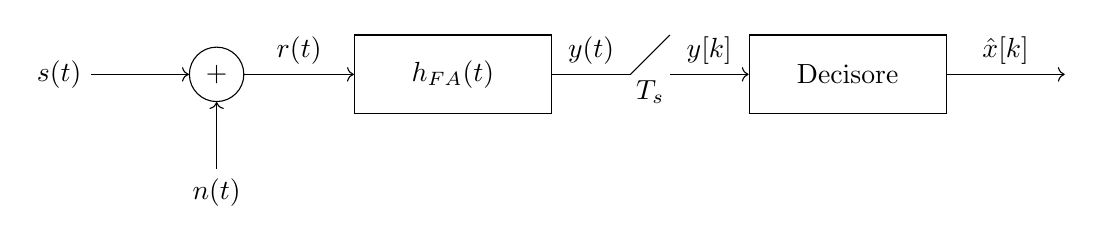
\begin{tikzpicture}[
            block/.style={rectangle, draw, minimum height=1cm, minimum width=2.5cm},
            node distance=2.5cm and 2.5cm,
            auto
        ]




        \node[block] (filter) {$h_{FA}(t)$};
        \node[right=of filter] (sampler) {};
        \node[block, right=of filter](decisore) {Decisore};

        \node (s) at (-5,0) {\(s(t)\)};
        \node[draw, circle] (plus) at (-3,0) {\(+\)};
        \node (n) at (-3,-1.5) {\(n(t)\)};

        \draw[->] (s) -- (plus);
        \draw[->] (n) -- (plus);
        %\draw[->] (plus) -- (channel);

        \draw[->] (plus) -- (filter) node[midway,above] {$r(t)$};

        \draw ([xshift=0]filter.east) -- ([xshift=1cm]filter.east) node[midway,above] {$y(t)$};
        \draw ([xshift=1cm]filter.east) -- ([xshift=1.5cm,yshift=0.5cm]filter.east) node[midway,below, yshift=-0.2cm] {$T_s$};

        \draw[->] ([xshift=1.5cm,yshift=0cm]filter.east) -- (decisore) node[midway,above] {$y[k]$};
        \draw[->] (decisore.east) -- ++(1.5,0) node[midway,above] {$\hat{x}[k]$};

    \end{tikzpicture}
\end{center}

\[
    s(t) = \sum_{k=-\infty}^{\infty} x[k] P(t - kT_s)
\]

\[
    P_E(M) = \frac{M-1}{M} \text{erfc} \left( \sqrt{\frac{3\cdot SNR \cdot \log_2 M}{M^2-1}} \right)
\]

\begin{center}

    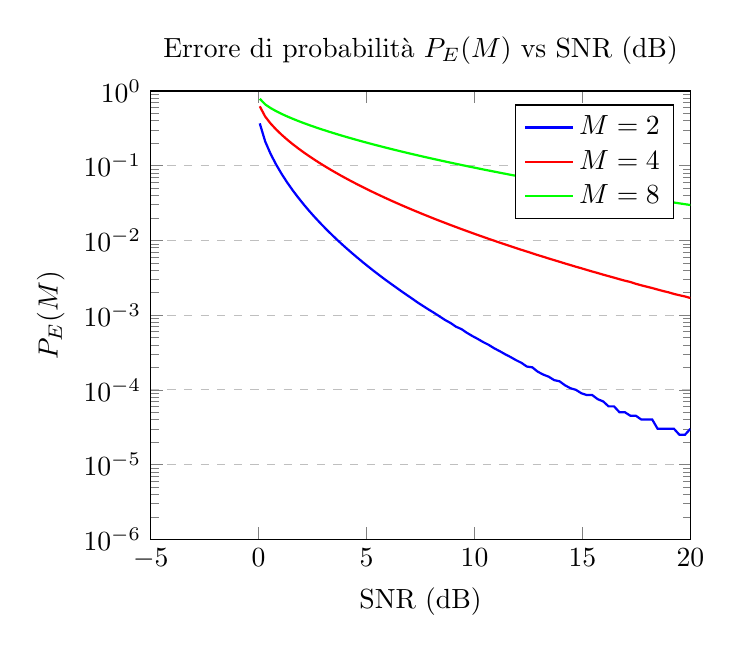
\begin{tikzpicture}
        \begin{axis}[
                title={Errore di probabilità $P_E(M)$ vs SNR (dB)},
                xlabel={SNR (dB)},
                ylabel={$P_E(M)$},
                xmin=-5, xmax=20,
                ymin=1e-6, ymax=1,
                ymode=log,
                legend pos=north east,
                ymajorgrids=true,
                grid style=dashed,
            ]

            % approximate erf(x) with tanh(1.2*x)
            \addplot[
                color=blue,
                mark=none,
                thick,
                domain=-5:20,
                samples=100,
            ] {0.5*(1-tanh(1.2*sqrt(x)))}; \addlegendentry{$M=2$}

            \addplot[
                color=red,
                mark=none,
                thick,
                domain=-5:20,
                samples=100,
            ] {0.75*(1-tanh(1.2*sqrt(2*x/5)))}; \addlegendentry{$M=4$}

            \addplot[
                color=green,
                mark=none,
                thick,
                domain=-5:20,
                samples=100,
            ] {0.875*(1-tanh(1.2*sqrt(x/7)))}; \addlegendentry{$M=8$}

        \end{axis}
    \end{tikzpicture}
\end{center}

Per SNR $> 10$ dB, utilizzando la codifica di Gray
\[
    P_E(b) \approx \frac{P_E(M)}{\log_2 M}
\]

Per una BPSK (2-PAM)
\[
    P_E(M) = P_E(b) = \frac{1}{2} \text{erfc}\left(\sqrt{\text{SNR}}\right)
\]

\paragraph{Dimostrazione}

Considerando le densità di probabilità $f_Y(y|x=1)$ e $f_Y(y|x=-1)$:

La probabilità di errore binario $P_E(b)$ è data dalla somma delle aree sotto le curve di $f_Y(y|x=1)$ e $f_Y(y|x=-1)$ dove queste si sovrappongono.



La densità di probabilità condizionata dato $x$ è:
\[
    P\{ \hat{x} = -1 | x = 1 \} = \int_{-\infty}^{\infty} f_Y(y | x = 1) \, dy
\]
\[
    f_Y(y | x = 1) = \frac{1}{\sqrt{2\pi \sigma_{n_u}^2}} \exp \left( -\frac{(y - h(0)x)^2}{2\sigma_{n_u}^2} \right) \quad \text{per} \quad x = 1
\]

Dopo il campionatore:
\[
    y[k] = x[k]\cdot h(0) + n_u[k]
\]

Dove la varianza del rumore è data da:
\[
    \sigma_{n_u}^2 = \frac{N_0}{2} E_{h_R} = \frac{N_0}{2} h(0)
\]

La densità spettrale di potenza del rumore bianco è:
\[
    S_w(f) = \frac{N_0}{2} \quad \Rightarrow \quad \text{DSP sul processo del rumore in ingresso è uguale in distribuzione } h_R(t)
\]

Il rapporto segnale-rumore (SNR) è:
\[
    SNR = \frac{h(0)^2}{\frac{N_0}{2} h(0)} = \frac{2 h(0)}{N_0}
\]

La probabilità condizionata dato $x$ è:
\[
    P\{ \hat{x} = -1 | x = 1 \} = 1 - Q\left( \frac{0 - h(0)}{\sqrt{\frac{N_0}{2} h(0)}} \right)
\]
\[
    = Q\left( \sqrt{\frac{2 h(0)}{N_0}} \right) = Q\left( \sqrt{SNR} \right) = \frac{1}{2} \text{erfc}\left( \sqrt{SNR} \right)
\]

Si può dimostrare per simmetria che:
\[
    P\{ \hat{x} = 1 | x = -1 \} = P\{ \hat{x} = -1 | x = 1 \} = \frac{1}{2} \text{erfc}\left( \sqrt{SNR} \right)
\]


Quindi:
\[
    P_E(b) = \frac{1}{2} \cdot \frac{1}{2} \text{erfc}\left( \frac{\sqrt{SNR}}{2} \right) + \frac{1}{2} \cdot \frac{1}{2} \text{erfc}\left( \frac{\sqrt{SNR}}{2} \right) = \frac{1}{2} \text{erfc}\left( \frac{\sqrt{SNR}}{2} \right)
\]

\paragraph{Presenza di ISI e rumore}

Il segnale ricevuto è:
\[
    y(t) = \sum_{k=-\infty}^{\infty} x[k] h(t - kT_s) + n_u(t)
\]

Dove:
\[
    h(t) = p(t) * c(t) * h_R(t)
\]
\[
    n_u(t) = n(t) * h_R(t)
\]

E il segnale al campionato è:
\[
    y[k] = x[k] \cdot h(0) + I[k] + n_u[k]
\]

Dove il termine di interferenza è dato da:
\[
    I[k] = \sum_{\substack{n=-\infty \\ n \neq k}}^{+\infty} x[n] h\left( (k-n)T_s \right)
\]

L'approccio da seguire è il seguente:
il filtro $h_R(t)$ deve essere allo stesso tempo quello che elimina l'ISI e che massimizza l'$SNR$. Questo problema può essere risolto progettando opportunamente $p(t)$ e $h_R(t)$.

\paragraph{Equalizzatore zero forcing}

Massimizza il SNR vincolando \( I[k] = 0 \) per ogni \( k \).  È un problema di massimizzazione vincolata per cui la soluzione non porta alla realizzazione del filtro adattato.

\begin{itemize}
    \item \( I[k] = 0 \) quando \( h(t) = h_{RC}(t) \), allora
          \[
              P(f) C(f) H_R(f) = H(f) = H_{RC}(f) e^{-j 2 \pi f T_s}
          \]
          per la causalità.

          Si pone quindi il problema di massimizzare il $SNR$ con il vincolo
          \[
              P(f) C(f) H_R(f) = H_{RC}(f) e^{-j 2 \pi f T_s}
          \]
\end{itemize}

Si può scrivere:
\[
    \left| P(f) \right| = \left| H_R(f) \right| = \sqrt{\frac{\left| H_{RC}(f) \right|}{\left| C(f) \right|}}
\]
\[
    \angle P(f) = \angle H_R(f) = - \pi f T_s - \frac{\angle C(f)}{2}
\]

N.B. Se \( C(f) = 1 \) (canale ideale) allora
\[
    P(f) = H_R(f) = \sqrt{H_{RC}(f)} e^{-j 2 \pi f T_s}
\]

Il valore di SNR in tal caso è:



\[
    SNR = \frac{E\left\{\left|X[k]\right|^2\right\} h^2(0)}{\frac{N_0}{2}
    \int_{-B_c}^{B_c} \frac{H_{RC}(f)}{C(f)}\, df }
\]

dove \( B_c \) è la banda del canale \( C(f) \), \( h(t) \) è la risposta all'impulso del canale ideale e $h(0)$ può essere visto come $
    \int_{-\infty}^{+\infty} H(f)\, df$.

\[
    E_s = P_s T_s = T_s \frac{M^2-1}{3}
\]

Se \( C(f) = 1 \) allora \( SNR = \frac{2 E_s}{N_0} \) e il filtro è adattato.

Il segnale ricevuto è:
\[
    r(t) = \sum_{k=-\infty}^{\infty} x[k] p(t - kT_s) + n(t)
\]
dove \( n(t) \) è il rumore bianco additivo gaussiano (AWGN).

La funzione di trasferimento del filtro ricevitore è:
\[
    h_{R}(f) = p (T_s - t)
\]
\[
    H_{R}(f) = P(f) e^{-j2\pi fT_s}
\]
\[
    H(f) = P^2(f) e^{-j2\pi fT_s} = H_{RC}(f) e^{-j2\pi fT_s}
\]

Riassumendo, il problema di eliminare l'ISI e massimizzare il SNR si risolve utilizzando il filtro sagomatore \( p(t) \) e quello di ricezione, \( h_R(t) \), realizzati con la radice di coseno rialzato.

Nel caso di canale ideale, la soluzione coincide con il filtro adattato.

\section*{Modulazione Numerica in Banda Passante}

\subsection*{Segnale Passa Banda}

Il segnale passa banda può essere espresso come:
\[
s(t) = a(t) \cos[2\pi f_0 t + \phi(t)]
\]
dove \( a(t) \) è l'inviluppo reale di \( s(t) \) (segnale passa-basso) e \( \phi(t) \) la fase di \( s(t) \).



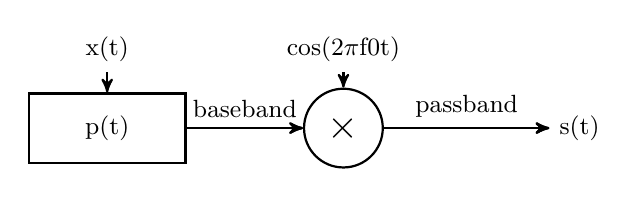
\begin{tikzpicture}[font=\small,>=stealth',thick, node distance=2cm]
\tikzstyle{block} = [rectangle, draw,
    text width=5em, text centered, minimum height=2.5em]
\tikzstyle{signal} = [draw,->]
\tikzstyle{modulator} = [circle, draw, inner sep=0pt, minimum size=1cm]

\node[block] (filter) {p(t)};
\node[modulator, right of=filter, node distance=3cm] (modulator) {\Large$\times$};
\node[above of=filter, node distance=1cm] (input) {x(t)};
\node[right of=modulator, node distance=3cm] (output) {s(t)};

\draw[signal] (input) -- (filter);
\draw[signal] (filter) -- (modulator);
\draw[signal] (modulator) -- (output);
\draw[signal] (filter) -- node[above] {baseband} (modulator);
\draw[signal] (modulator.east) -- node[above] {passband} (output);

\node[above of=modulator, node distance=1cm] (carrier) {cos(2$\pi$f0t)};
\draw[signal] (carrier) -- (modulator);

\end{tikzpicture}


Espandendo l'inviluppo complesso di \( s(t) \), otteniamo:
\[
s(t) = \Re\left\{ a(t) e^{j[2\pi f_0 t + \phi(t)]} \right\}
\]
\[
= \Re\left\{ a(t) \cos[2\pi f_0 t + \phi(t)] + j \cdot a(t) \sin[2\pi f_0 t + \phi(t)] \right\}
\]
\[
= a(t) \cos[2\pi f_0 t + \phi(t)] = \Re\left\{ \tilde{a}(t) e^{j2\pi f_0 t} \right\}
\]
dove \( \tilde{a}(t) \) è l'inviluppo complesso di \( s(t) \).



















\begin{tikzpicture}[>=Stealth, 
    block/.style={draw, rectangle, minimum height=2em, minimum width=3em},
    sum/.style={draw, circle, node distance=1cm},
    node distance=2cm and 3cm
]
    % Nodes
    \node[block] (pfilter) {$p(t)$};
    \node[sum, right of=pfilter] (mixer) {$\times$};
    \node[right= of mixer] (output) {$s(t)$};
    \node[above= of mixer] (cosine) {$\cos(2\pi f_0 t)$};
    \node[left= of pfilter] (input) {$x(t)$};
    
    % Lines
    \draw[->] (input) -- (pfilter);
    \draw[->] (pfilter) -- (mixer);
    \draw[->] (mixer) -- (output);
    \draw[->] (cosine) -- (mixer);

    % Lower part with s tilde
    \node[block, below= of pfilter] (pfilter2) {$p(t)$};
    \node[sum, right of=pfilter2] (mixer2) {$\times$};
    \node[right= of mixer2] (output2) {$\tilde{s}(t)$};
    \node[above= of mixer2] (exponential) {$e^{j2\pi f_0 t}$};
    \node[left= of pfilter2] (input2) {$\tilde{x}(t)$};
    
    % Lines for lower part
    \draw[->] (input2) -- (pfilter2);
    \draw[->] (pfilter2) -- (mixer2);
    \draw[->] (mixer2) -- (output2);
    \draw[->] (exponential) -- (mixer2);
    
    % Draw the constellation diagram
    \begin{scope}[shift={($(output2.south east)+(3cm,-1cm)$)},scale=0.5]
        \draw[->] (-4,0) -- (4,0) node[below] {$\Re$};
        \draw[->] (0,-3) -- (0,3) node[left] {$\Im$};
        
        % Points in the constellation
        \foreach \x in {-3,-1,1,3}
            \fill[orange] (\x,0) circle (5pt);
            
        % Label for n=4
        \node[below] at (3,0) {$n=4$};
    \end{scope}
\end{tikzpicture}








% Definizione di M-PAM
\[
M-PAM \quad \Rightarrow \quad \text{simboli:} \quad A_s = \{\alpha_1, \dots, \alpha_M\}
\]
\[
\alpha = 2c - 1 - M
\]
\[
p(t) = \text{impulso in TX}
\]

% Definizione del segnale s(t)
\[
s(t) = \sum_{n=-\infty}^{\infty} x(n) p(t - nT_s) \cos(2\pi f_c t)
\]

% Diagramma segnale
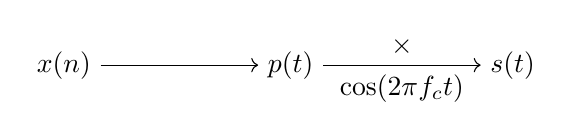
\begin{tikzpicture}
\node (x) at (0,0) {$x(n)$};
\node[right=2cm of x] (p) {$p(t)$};
\node[right=2cm of p] (s) {$s(t)$};
\draw[->] (x) -- (p);
\draw[->] (p) -- (s) node[midway,above] {$\times$} node[midway,below] {$\cos(2\pi f_c t)$};
\end{tikzpicture}

% Altre espressioni del segnale
\[
\tilde{S}(t) = \sum_{n=-\infty}^{\infty} x(n) p(t - nT_s)
\]
\[
\tilde{s}(t) = \Re\{\tilde{S}(t) e^{j2\pi f_c t}\}
\]
\[
= \Re \left\{ \sum_{n=-\infty}^{\infty} x(n) p(t - nT_s) e^{j2\pi f_c t} \right\}
\]
\[
= \sum_{n=-\infty}^{\infty} x(n) p(t - nT_s) \cos(2\pi f_c t) + j \sin(2\pi f_c t)
\]

% Diagramma dei simboli
\begin{tikzpicture}
\draw[->] (-3.5,0) -- (3.5,0) node[anchor=west] {$\Re$};
\draw[->] (0,-2) -- (0,2) node[anchor=south] {$\Im$};
\foreach \x in {-3,...,3}
  \draw (\x,0.1) -- (\x,-0.1) node[anchor=north] {$\x$};
\foreach \y in {-1,1}
  \draw (0.1,\y) -- (-0.1,\y) node[anchor=east] {$\y$};
% Aggiungere punti qui se necessario
\end{tikzpicture}
\noindent Modulazione di fase PSK (Phase Shift Keying):

% Definizione del segnale s(t)
\begin{flalign}
& s_c(t) = p(t) \cos(2\pi f_0 t + \theta_i) && \text{(simbolo $i$-esimo)} & \\
& \theta_i = \frac{2\pi}{M}(i-1) && \text{per $i = 1, \ldots, M$} &
\end{flalign}

\noindent Espansione del segnale s(t) come sommatoria:

\begin{flalign}
& s(t) = \sum_{n=-\infty}^{\infty} p(t - nT_s) \cos(2\pi f_0 t + \theta_i(n)) & \\
& \theta_i(n) \in A_s = \{\theta_1, \ldots, \theta_M\} &
\end{flalign}

\noindent Definizione del segnale modulato in fase $\tilde{s}_c(t)$:

\begin{flalign}
& \tilde{s}_c(t) = p(t) e^{j\theta_i} & \\
& \tilde{s}_c(t) = \Re\{p(t) e^{j\theta_i} e^{j2\pi f_0 t}\} & \\
& \phantom{\tilde{s}_c(t)} = \Re\{p(t) e^{j(2\pi f_0 t + \theta_i)}\} & \\
& \phantom{\tilde{s}_c(t)} = p(t) \cos(2\pi f_0 t + \theta_i) &
\end{flalign}

\noindent Definizione di $x(n)$ basata su $\theta_n$:

\begin{flalign}
& x(n) = e^{j\theta_n} &
\end{flalign}
% Equations arranged in a row
\noindent
\begin{minipage}{.5\linewidth}
\begin{equation*}
    s(t) = \Re \{ s(t) e^{j 2\pi f_0 t} \}
\end{equation*}
\begin{equation*}
    s(t) \approx \sum_{n=-\infty}^{\infty} s_n e^{j \Omega_n}
\end{equation*}
\end{minipage}%
\begin{minipage}{.5\linewidth}
\begin{equation*}
    s(t) = \Re \left\{ \sum_{n=-\infty}^{\infty} p(t-nT_s) e^{j (2\pi f_0 t + \Omega_n)} \right\}
\end{equation*}
\end{minipage}

% Another row of equations
\noindent
\begin{minipage}{.5\linewidth}
\begin{equation*}
    \approx \sum_{n=-\infty}^{\infty} p(t+nT_s) \cos(2\pi f_0 t + \Theta_n)
\end{equation*}
\end{minipage}%
\begin{minipage}{.5\linewidth}
\begin{equation*}
    S_i(t) = A_{I_i} p(t) \cos(2\pi f_0 t) - A_{Q_i} p(t) \sin(2\pi f_0 t)
\end{equation*}
\end{minipage}

% TikZ Diagram in a row with QAM explanation
\noindent
\begin{minipage}[c]{0.3\linewidth}
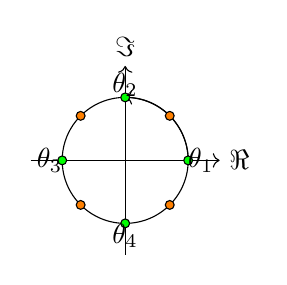
\begin{tikzpicture}[scale=0.8]
    \draw[->] (-1.5,0) -- (1.5,0) node[right] {$\Re$};
    \draw[->] (0,-1.5) -- (0,1.5) node[above] {$\Im$};
    \draw (0,0) circle (1cm);
    \draw[->] (1,0) arc (0:90:1cm);
    \foreach \angle/\label in {0/\theta_1, 90/\theta_2, 180/\theta_3, 270/\theta_4}{
      \draw[fill=green] (\angle:1cm) circle (2pt);
      \node at (\angle:1.2cm) {$\label$};
    }
    \foreach \angle in {45,135,225,315}{
      \draw[fill=orange] (\angle:1cm) circle (2pt);
    }
\end{tikzpicture}
\end{minipage}%
\begin{minipage}[c]{0.7\linewidth}
\begin{equation*}
    \frac{A_{I_i}}{A_{Q_i}} \text{ -- verso e ampiezza della modulazione}
\end{equation*}
\begin{equation*}
    i \text{ -- indice del simbolo } x(t)
\end{equation*}
\end{minipage}




% Start of the content
\[
A^c_i = \text{componente in fase di } x(t)
\]
\[
A^s_i = \text{componente in quadratura di } x(t)
\]

\[
s^c_i(t) = (A^c_i + j A^s_i) p(t)
\]

\[
\Re\{s^c_i(t) e^{j2\pi f_0t}\} = \Re\{(A^c_i + A^s_i) p(t) e^{j2\pi f_0t}\}
\]

\[
= \Re\{A^c_i p(t) e^{j2\pi f_0t} + j A^s_i p(t) e^{j2\pi f_0t}\}
\]

\[
= \Re\{A^c_i p(t) \cos(2\pi f_0t) + j A^c_i p(t) \sin(2\pi f_0t) + A^s_i p(t) \cos(2\pi f_0t) - A^s_i p(t) \sin(2\pi f_0t)\}
\]

\[
= A^c_i p(t) \cos(2\pi f_0t) - A^s_i p(t) \sin(2\pi f_0t)
\]

\[
s(t) = \sum_{n=-\infty}^{+\infty} x_n p(t-nT_s) \cos(2\pi f_0t) - x_s p(t-nT_s) \sin(2\pi f_0t)
\]

\[
s(t) = \Re\{\sum_{n=-\infty}^{+\infty} x_n p(t-nT_s)e^{j2\pi f_0 t}\}
\]

\[
    x[n] = x_c[n] + jx_s[n]
\]



\section*{Modulazione QAM}



\paragraph*{Modulazione QAM (Quadrature Amplitude Modulation)}


\begin{equation*}
    S_i(t) = A_{I_i} p(t) \cos(2\pi f_0 t) - A_{Q_i} p(t) \sin(2\pi f_0 t)
\end{equation*}

% TikZ Diagram in a row with QAM explanation
\noindent
\begin{minipage}[c]{0.3\linewidth}

\end{minipage}%
\begin{minipage}[c]{0.7\linewidth}
    \begin{equation*}
        \frac{A_{I_i}}{A_{Q_i}} \text{ -- verso e ampiezza della modulazione}
    \end{equation*}
    \begin{equation*}
        i \text{ -- indice del simbolo } x(t)
    \end{equation*}
\end{minipage}




% Start of the content
\[
    A^c_i = \text{componente in fase di } x(t)
\]
\[
    A^s_i = \text{componente in quadratura di } x(t)
\]

\[
    s^c_i(t) = (A^c_i + j A^s_i) p(t)
\]

\[
    \Re\{s^c_i(t) e^{j2\pi f_0t}\} = \Re\{(A^c_i + A^s_i) p(t) e^{j2\pi f_0t}\}
\]

\[
    = \Re\{A^c_i p(t) e^{j2\pi f_0t} + j A^s_i p(t) e^{j2\pi f_0t}\}
\]

\[
    = \Re\{A^c_i p(t) \cos(2\pi f_0t) + j A^c_i p(t) \sin(2\pi f_0t) + A^s_i p(t) \cos(2\pi f_0t) - A^s_i p(t) \sin(2\pi f_0t)\}
\]

\[
    = A^c_i p(t) \cos(2\pi f_0t) - A^s_i p(t) \sin(2\pi f_0t)
\]

\[
    s(t) = \sum_{n=-\infty}^{+\infty} x_n p(t-nT_s) \cos(2\pi f_0t) - x_s p(t-nT_s) \sin(2\pi f_0t)
\]

\[
    s(t) = \Re\{\sum_{n=-\infty}^{+\infty} x_n p(t-nT_s)e^{j2\pi f_0 t}\}
\]

\[
    x[n] = x_c[n] + jx_s[n]
\]



\begin{align*}
    x(t)   & = x_c(t) + j \cdot x_s(t)                \\
    x_c(t) & = \Re\{p(t)\} \quad x_s(t) = \Im\{p(t)\}
\end{align*}

% Qui viene rappresentato il diagramma di flusso della modulazione QAM
\begin{tikzpicture}
    % Definire i nodi e i percorsi qui
\end{tikzpicture}

\[
    x(t) = x_c(t) \cos(2\pi f_ct) - x_s(t) \sin(2\pi f_ct)
\]

% Diagramma dei punti della costellazione QAM
\begin{tikzpicture}
    \draw [<->] (0,2) node (yaxis) [above] {$\Im$}
    |- (2,0) node (xaxis) [right] {$\Re$};
    \draw (-1,0) -- (1,0);
    \draw (0,-1) -- (0,1);
    \foreach \x/\y in {-1/1, 1/1, -1/-1, 1/-1}
    \draw[fill=orange] (\x,\y) circle (2pt);
\end{tikzpicture}

\[
    \Gamma = \Gamma_c \cap \Gamma_s
\]

\begin{align*}
    A^\Gamma & = \{\alpha^\Gamma_c, \overline{\alpha^\Gamma_c}\} \\
    A^\Gamma & = \{\alpha^\Gamma_s, \overline{\alpha^\Gamma_s}\}
\end{align*}

\[
    A^c \rightarrow \alpha^c = 2c - 1 - \Gamma_c \quad A^s \rightarrow \alpha^s = 2c - 1 - \Gamma_s
\]



\end{document}



